\IEEEPARstart{A}{l} igual que con el experimento previo, segu\'imos utilizando
la metodolog\'ia de experimentaci\'on ya explicada. Con lo cual se ahondar\'a
menos en explicaciones de como leer los graficos y simplemente se pasar\'a a
analizar los resultados. M\'as a\'un en este experimento, donde los resultados
obtenidos fueron muy similares a los del experimento para \emph{camara fija,
im\'agen fija} (\ref{subsec:fija-fija}).

%---------------------------------------------------------------
\subsubsection{Spline}

\begin{figure}[H]
    \centering
    \subfloat[][ECM para 10 frames interpolados]{
        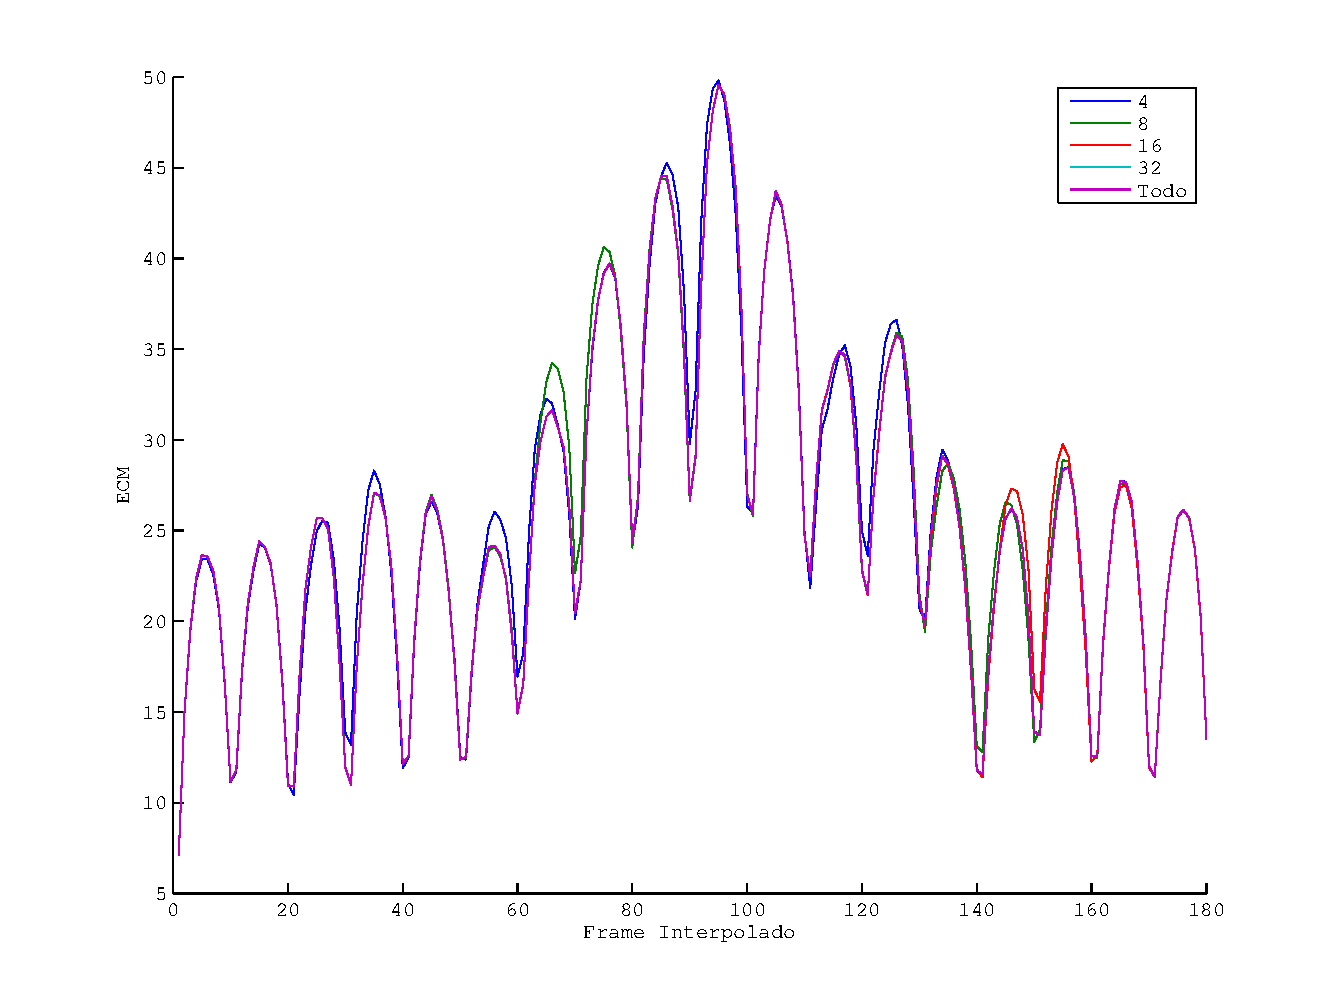
\includegraphics[width=.5\textwidth]{mse_spline-camara_movil-imagen_fija-k10.pdf}
        \label{subfig:movil-fija_spline-mse-k10}
    }
    \subfloat[][PSNR para 10 frames interpolados]{
        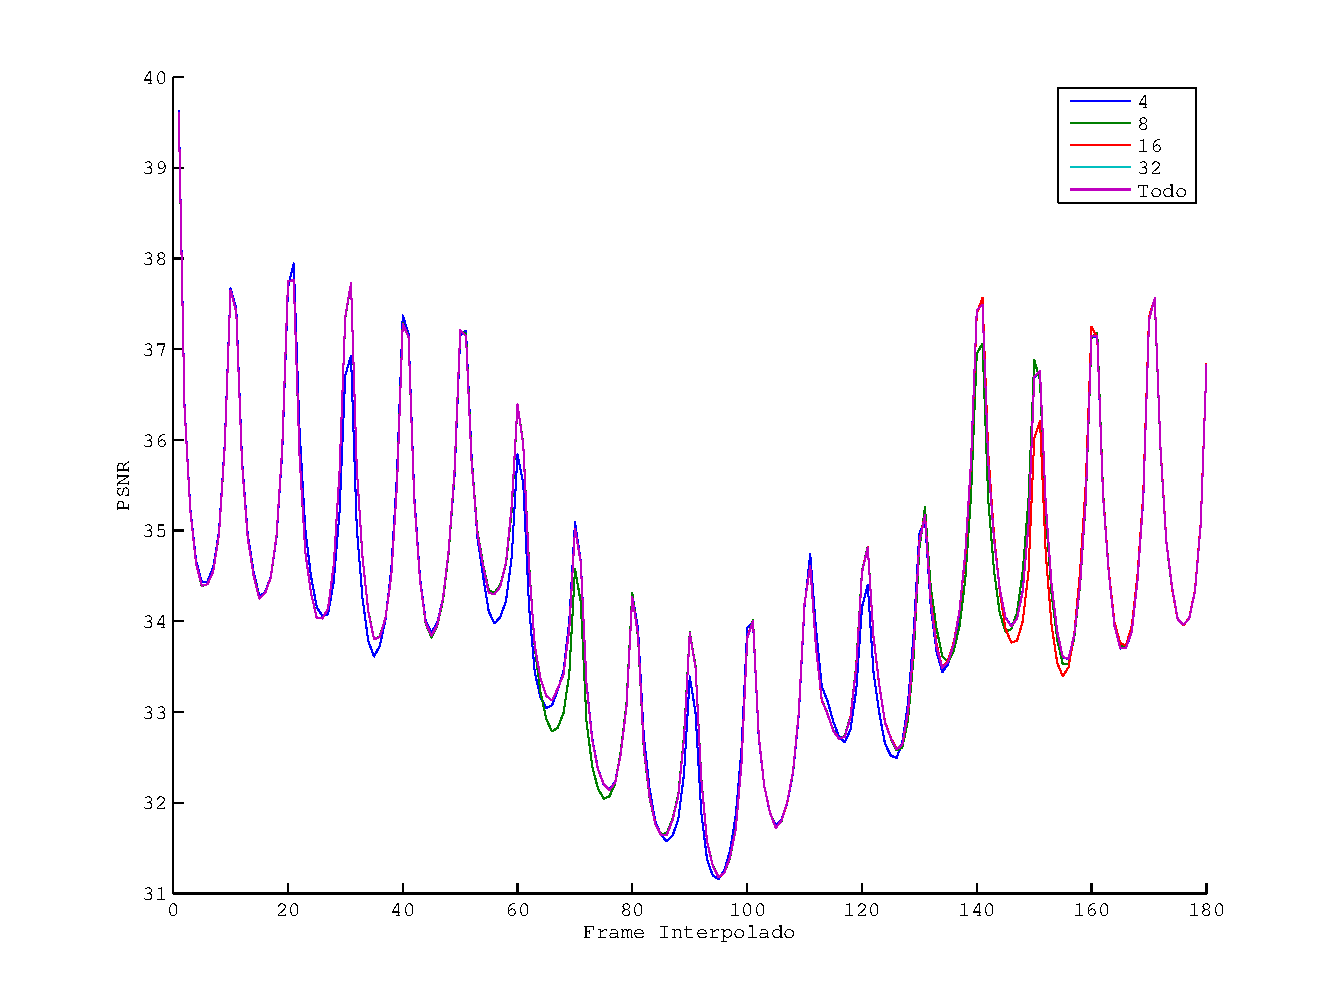
\includegraphics[width=.5\textwidth]{psnr_spline-camara_movil-imagen_fija-k10.pdf}
        \label{subfig:movil-fija_spline-psnr-k10}
    }
    \caption{Comparativa tama\~no de bloque para 10 frames interpolados}
    \label{fig:movil-fija_spline-bloques}
\end{figure}

\begin{figure}[H]
    \centering
    \subfloat[][Valor medio, Desv\'io Est\'andar, M\'aximo y M\'inimo\label{tbl:movil-fija_spline_k10}]{
        \footnotesize
        \setlength{\tabcolsep}{3pt}
        \begin{tabular}{|l|r|r|r|r|}
            \hline
            \textbf{Bloque}& \textbf{Mean}& \textbf{Std}& \textbf{M\'ax}& \textbf{M\'in}\\
            \hline\hline
            4&26.1529& 9.0556& 49.8088& 7.0709\\
            8&26.0635& 9.0431& 49.5983& 7.1123\\
            16&25.9427& 8.9583& 49.5654& 7.1070\\
            32&25.8502& 8.9852& 49.5525& 7.1070\\
            Entero&25.8502& 8.9852& 49.5525& 7.1070\\
            \hline
        \end{tabular}
    }\hspace{10pt}
    \subfloat[][Diferencia M\'axima\label{tbl:movil-fija_dif_spline_k10}]{
        \footnotesize
        \setlength{\tabcolsep}{3pt}
        \begin{tabular}{|l|r|r|r|r|r|}
            \hline
            \textbf{Bloque}& \textbf{vs 4}& \textbf{vs 8}& \textbf{vs 16}& \textbf{vs 32}& \textbf{vs Entero}\\
            \hline\hline
            \textbf{4}&0& 3.6585& 3.5640& 3.5744& 3.5744\\
            \textbf{8}&3.7434& 0& 3.2126& 3.2126& 3.2126\\
            \textbf{16}&2.6864& 3.8550& 0& 2.5903& 2.5903\\
            \textbf{32}&1.5005& 1.2646& 0.7720& 0& 0\\
            \textbf{Entero}&1.5005& 1.2646& 0.7720& 0& 0\\
            \hline
        \end{tabular}
    }
    \caption{Comparativa ECM seg\'un tama\~no de bloque}
    \label{fig:movil-fija_stats-spline_k10}
\end{figure}

\par Los resultados obtenidos en cuanto al an\'alisis del tama\~no de bloque
son similares a los de la secci\'on \ref{subsec:fija-fija}. Se observa en la
figura \ref{fig:movil-fija_spline-bloques} que el ECM/PSNR se encuentra muy
solapado para cualquier tama\~no de bloque (y tambi\'en para todas las variantes
de cantidad de frames interpolados, cuyos gr\'aficos no consideramos pertinentes
exponer ya que muestran el mismo comportamiento), d\'andonos a entender que
el tama\~no del bloque no influye significativamente para este video (el
an\'alisis es el mismo que el expueto para el caso de la secci\'on
\ref{subsubsec:fija-fija_spline})

\par A su vez, al observar las tablas de la figura
\ref{fig:movil-fija_stats-spline_k10} vemos como los valores est\'adisticos
para todos los tama\~nos de bloques son similares (cuadro
\ref{tbl:movil-fija_spline_k10}) y que existe una ligera ventaja para los
tama\~nos de bloque mayores al analizar la diferencia m\'axima de los ECM para
un mismo frame (cuadro \ref{tbl:movil-fija_dif_spline_k10}), es decir, el
caso/frame en que la estimaci\'on de los tama\~nos de bloque ''grandes''
estiman mucho peor que los peque\~nos es ligeramente menor que el caso donde
los tama\~nos peque\~nos estiman mucho peor que los grandes. De hecho,
observamos que para un tama\~no de bloque de 32 frames, la diferencia para con
tomar el video entero es 0, indicando que ya a partir de un tama\~no de bloque
de 32 frames ser\'ia lo mismo tomar cualquier otro tama\~no (esto es
simplemente una nueva hip\'otesis, que por limitantes de tiempo no pudo ser
evaluada).

\par Pasando a un an\'alisis m\'as enfocado en lo que ocurre respecto de la
cantidad de frames interpolados, se presentan los ECM en funci\'on de los frames
interpolados en las figuras \ref{fig:movil-fija_spline-frames-interpolados} y
\ref{subfig:movil-fija_spline-mse-k10}.

\begin{figure}[H]
    \centering
    \subfloat[][ECM para 1 frame interpolado]{
        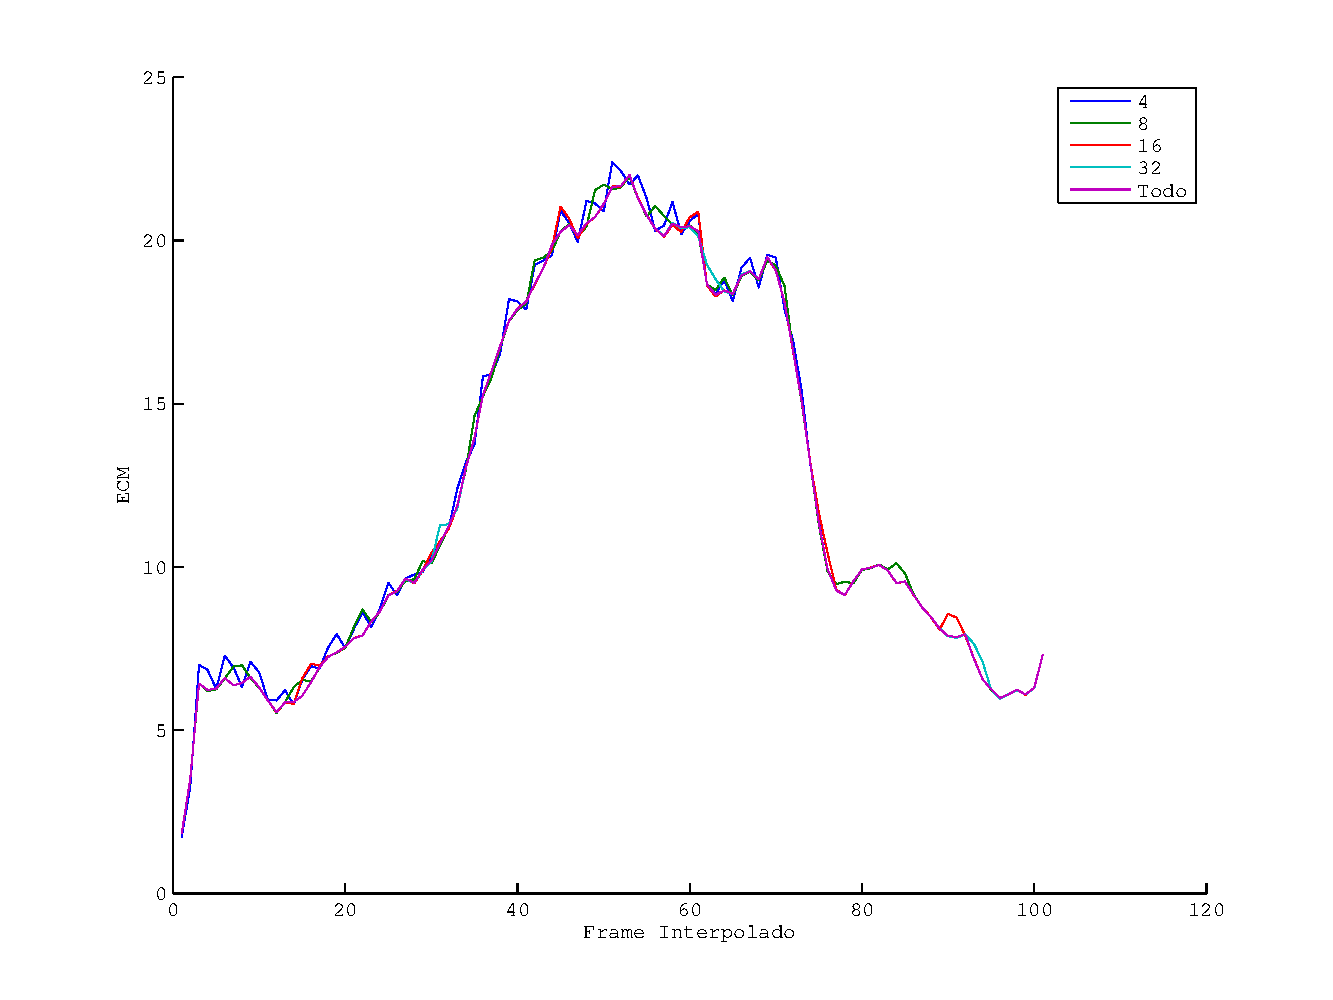
\includegraphics[width=.5\textwidth]{mse_spline-camara_movil-imagen_fija-k1.pdf}
        \label{subfig:movil-fija_spline-mse-k1}
    }
    \subfloat[][ECM para 5 frames interpolados]{
        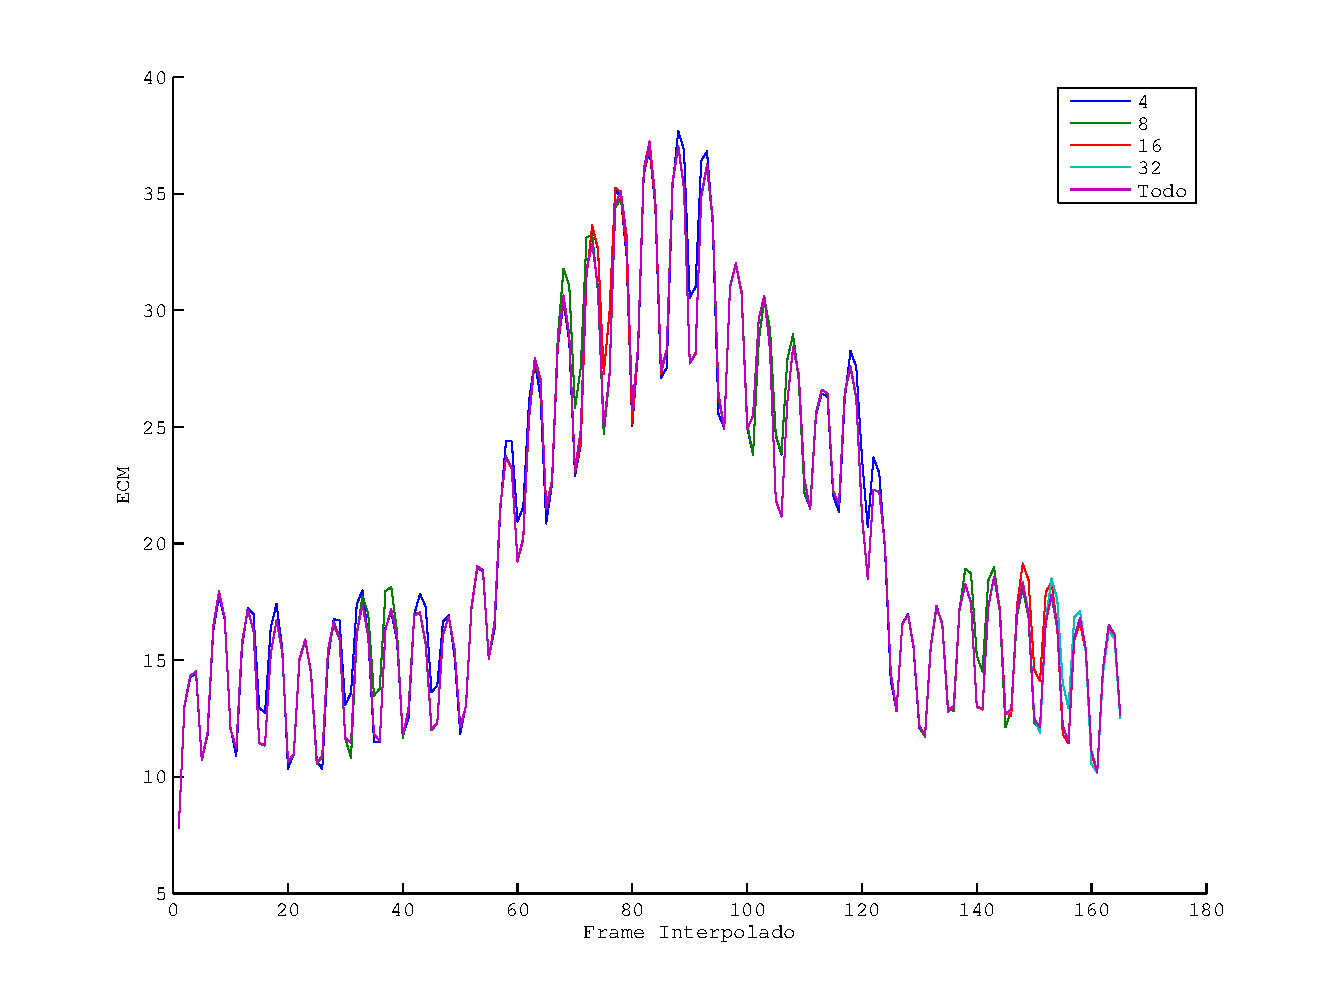
\includegraphics[width=.5\textwidth]{mse_spline-camara_movil-imagen_fija-k5.pdf}
        \label{subfig:movil-fija_spline-mse-k5}
    }
    \caption{Comparativa seg\'un cantidad de bloques interpolados}
    \label{fig:movil-fija_spline-frames-interpolados}
\end{figure}

\par M\'as all\'a de la obvia diferencia de escalas en el eje de los frames
interpolados\footnote{Eje $x$, coloquialmente hablando.} debido a la cantidad
total de frames interpolados por cada variante, se observa que la progresi\'on
del ECM es m\'as oscilante y c\'iclica a medida que se interpolan m\'as frames.

\par Mientras que para la interpolaci\'on de 1 frame\footnote{O 2 frames, si
bien dicha gr\'afica no ha sido expuesta, sus resultados son equivalentes en
cuanto a lo que est\'a siendo analizado al caso de la interpolaci\'on de 1
frame.} muestra un comportamiento m\'as ''suave'', si se quiere, las
evoluciones para los casos de 5 y 10 frames muestran constantes subas y bajas
de error para frames interpolados cercanos. Estas subas y bajas se corresponden
con la cercan\'ia del frame interpolado respecto de los frames utilizados para
calcular el spline (es decir, los frames originales con los que se realiz\'o la
interpolaci\'on).

\par Si se observan los valores est\'adisticos del ECM (figura
\ref{fig:movil-fija_spline-mse_estadisticas}) se observar\'a un comportamiento
no s\'olo acorde a la conclusi\'on de que el tama\~no de bloque no afecta
sustancialmente los resultados, sino que adem\'as son consistentes con las
hip\'otesis planteadas.

\par Se ve aqu\'i que cualquiera de las caracter\'isticas observadas (valor
medio, desv\'io est\'andar, m\'aximo o m\'inimo) se mantienen en valores
simlares sin importar el tama\~no de bloque, y que a su vez al tener que
interpolar una mayor cantidad de frames mayor es el ECM correspondiente al
proceso (lo cual es una de nuestras hip\'otesis). La \'unica excepci\'on a esto
es el ECM m\'inimo para el caso de 5 y 10 frames interpolados, donde
seguramente por cuestiones relacionadas con el movimiento de la camara existe
alg\'un frame que al ser utilizado en la interpolaci\'on de 5 frames y no ser
utilizado (probablemente) en la de 10 frames llevan al m\'etodo a estimar un (o
unos) frames de mejor manera. Es decir, no necesariamente tener m\'as frames
originales (o menos frames a interpolar\footnote{Siempre en el contexto de la
metodolog\'ia de experimentaci\'on utilizada, donde se remueven frames y luego
se interpolan para poder ser comparados.}) llevar\'a al m\'etodo a tener un
menor ECM m\'inimo (una cota para lo mejor que puede aproximar), aunque si
vemos que en el ECM medio esto s\'i se cumple.

\begin{figure}[H]
    \centering
    \subfloat[][Valor Medio]{
        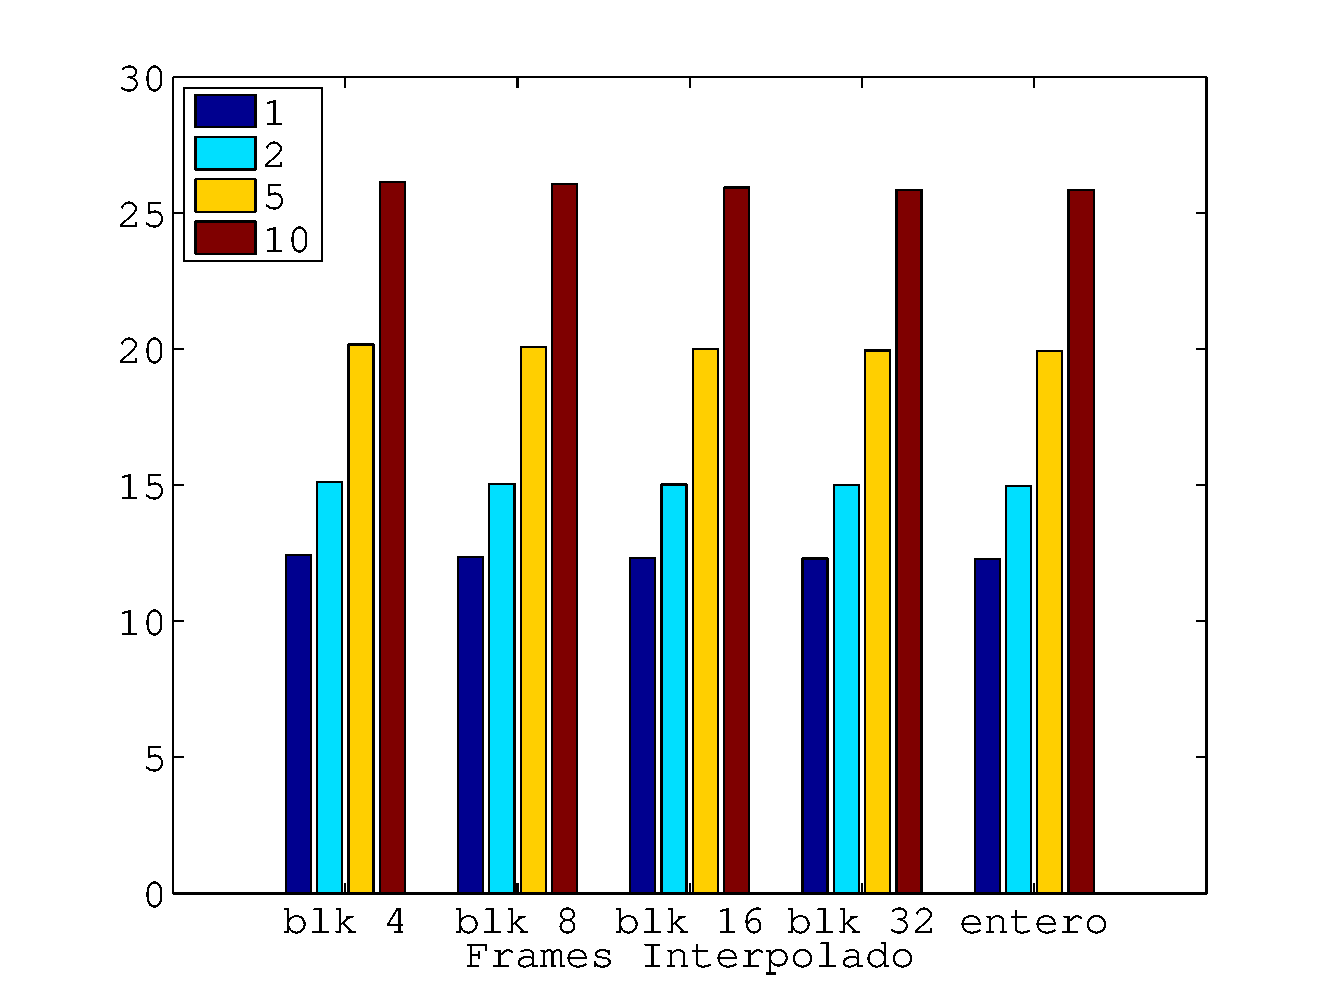
\includegraphics[width=.5\textwidth]{camara_movil-imagen_fija-mean_spline.pdf}
    }
    \subfloat[][Desv\'io Est\'andar]{
        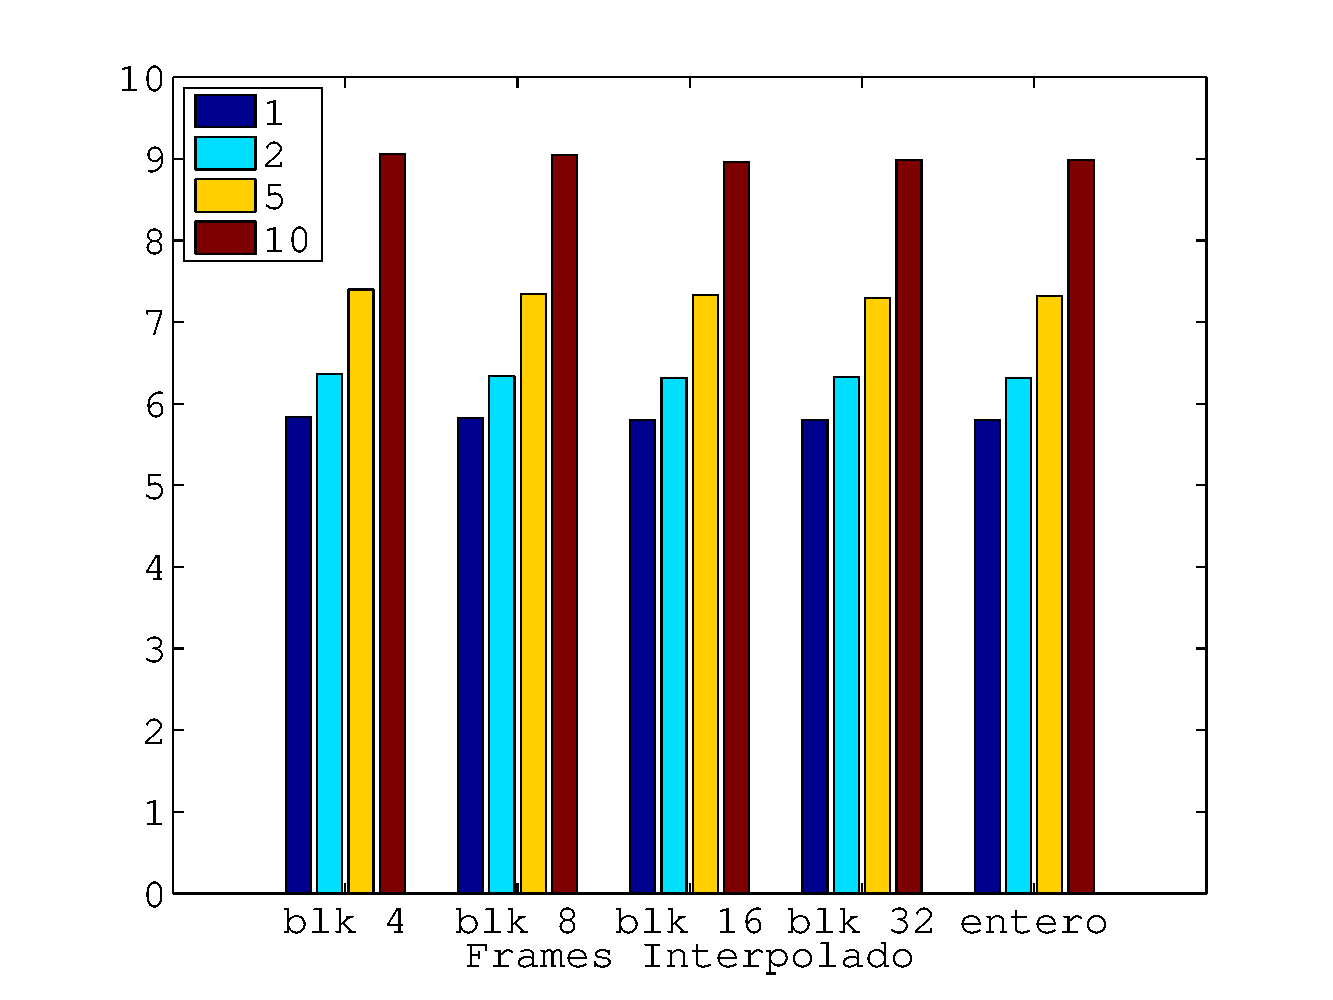
\includegraphics[width=.5\textwidth]{camara_movil-imagen_fija-std_spline.pdf}
    }\\
    \subfloat[][M\'aximo]{
        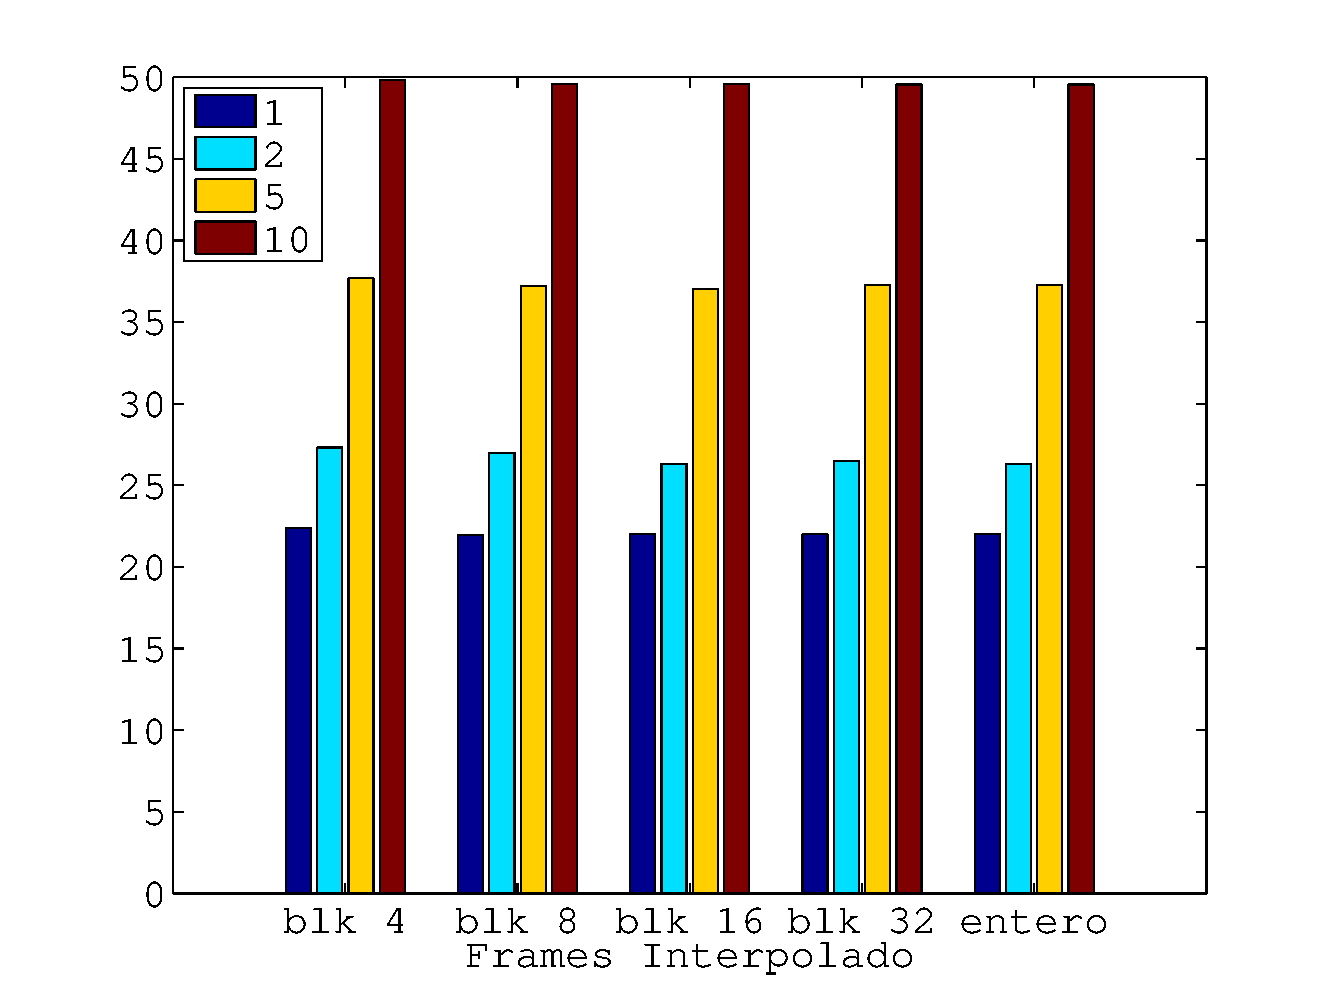
\includegraphics[width=.5\textwidth]{camara_movil-imagen_fija-max_spline.pdf}
    }
    \subfloat[][M\'inimo]{
        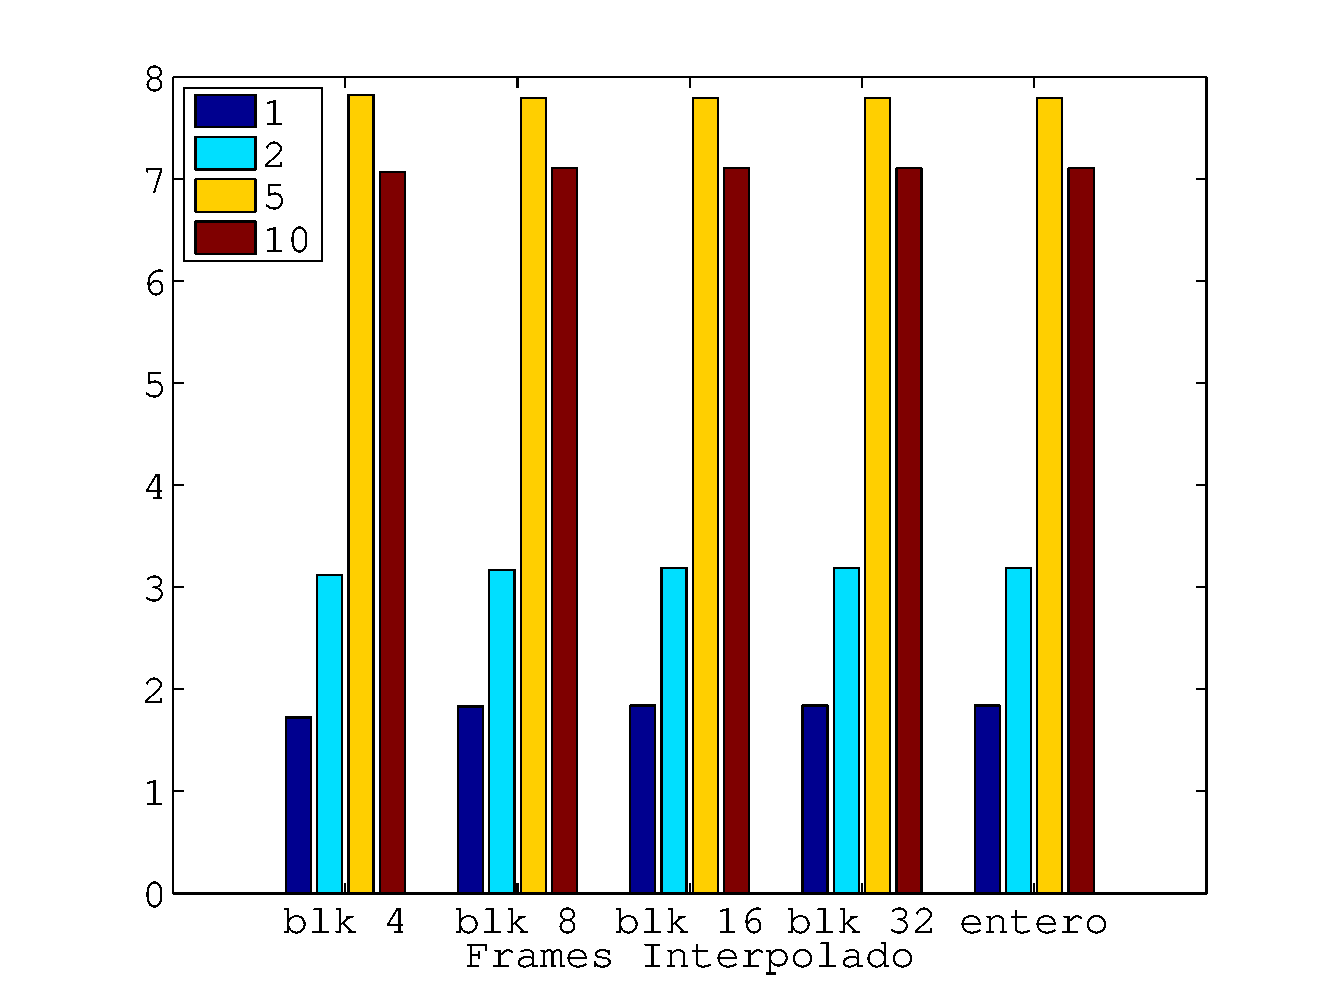
\includegraphics[width=.5\textwidth]{camara_movil-imagen_fija-min_spline.pdf}
    }
    \caption{Est\'adisticas ECM Seg\'un Frames Interpolados - Spline}
    \label{fig:movil-fija_spline-mse_estadisticas}
\end{figure}

\begin{figure}[H]
    \centering
    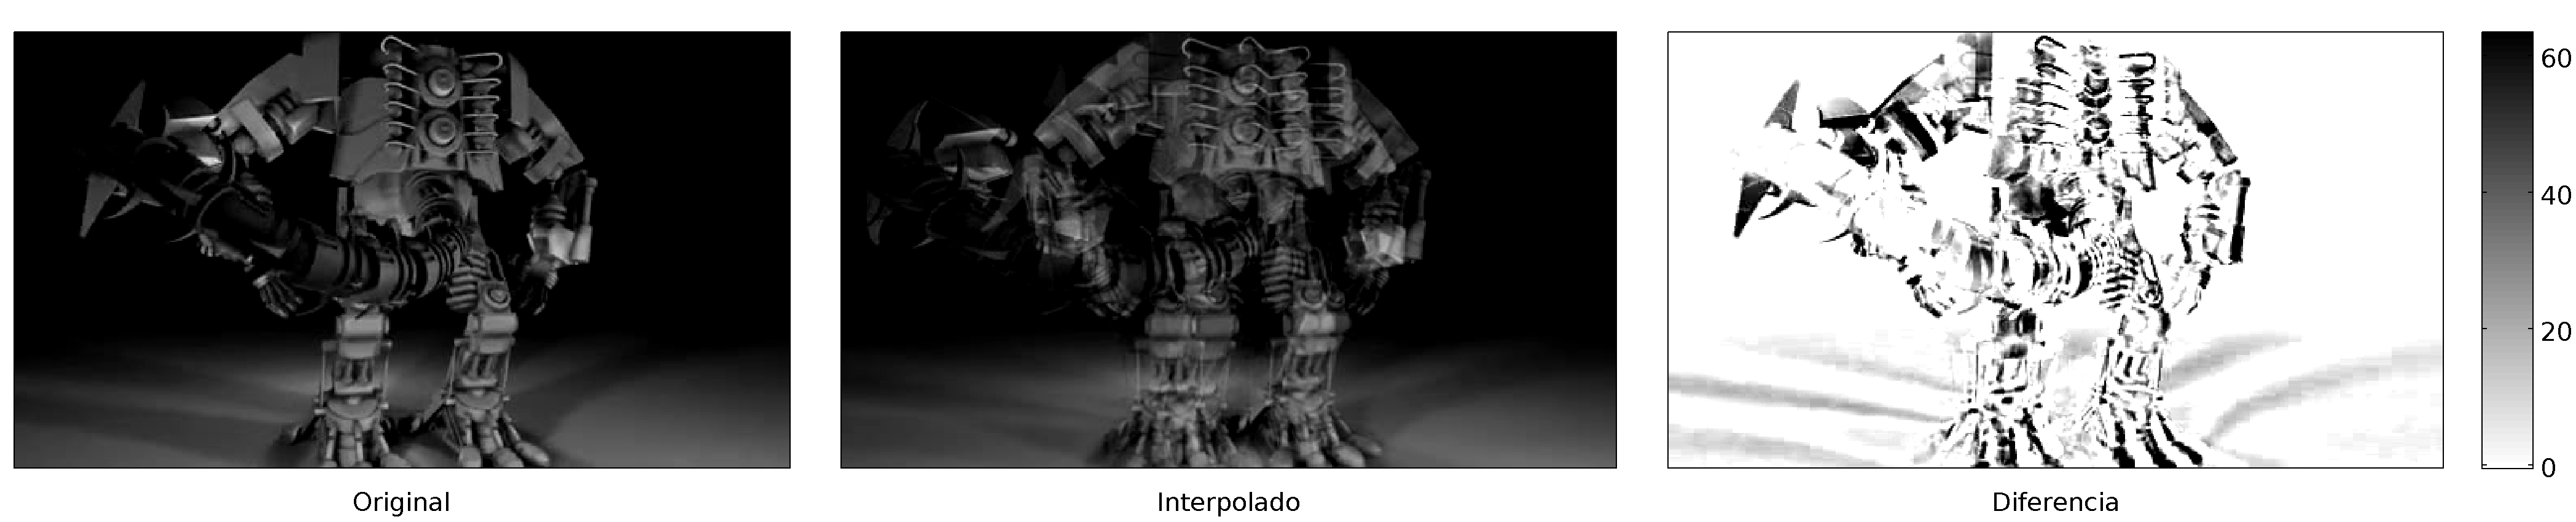
\includegraphics[width=\textwidth]{camara_movil-imagen_fija-spline-k10.png}
    \label{fig:movil-fija_spline-heatmap}
    \caption{Regi\'on peor aproximada por la interpolaci\'on por spline}
\end{figure}

\par Por \'ultimo, pasamos a analizar el video comparativo de la diferencia
entre los frames originales y sus
estimaciones\footnote{\url{https://drive.google.com/open?id=0B0RfkWV-4-XqT1NaU191cWRKOUE}}
~, para lo cual se utiliz\'o (siguiendo un razonamiento ya utilizado en el marco
de la experimentaci\'on) el caso de 10 frames interpolados para tama\~no de
bloque equivalente a todo el v\'ideo (ya que con estos par\'ametros obtenemos
el mayor desv\'io est\'andar y ECM medio). Se expone en la figura
\ref{fig:movil-fija_spline-heatmap} una captura representativa de dicho video.

\par Lo observado en dicho video no difiere de lo visto en el caso previo ni de
las hip\'otesis planteadas. Se ve que los puntos/regiones donde se genera el
error en la estimaci\'on/interpolaci\'on corresponden a los puntos del objeto
est\'atico (en el caso del video siendo analizado, una animaci\'on 3D de un
robot humanoide\footnote{Transformer.}) cambiando su posici\'on a medida que
progresan los frames debido al movimiento de la c\'amara. De hecho, esto puede
interpretarse como el objeto movi\'endose, y la c\'amara quedando est\'atica,
en cuyo caso vemos nuevamente que lo interpolado de manera menos precisa por el
m\'etodo se corresponde con el movimiento, o m\'as anal\'iticamente, con los
puntos representados ''desplaz\'andose'' por el cuadro.

%---------------------------------------------------------------
\subsubsection{Interpolaci\'on Lineal}

\begin{figure}[H]
    \centering
    \subfloat[][Valor Medio]{
        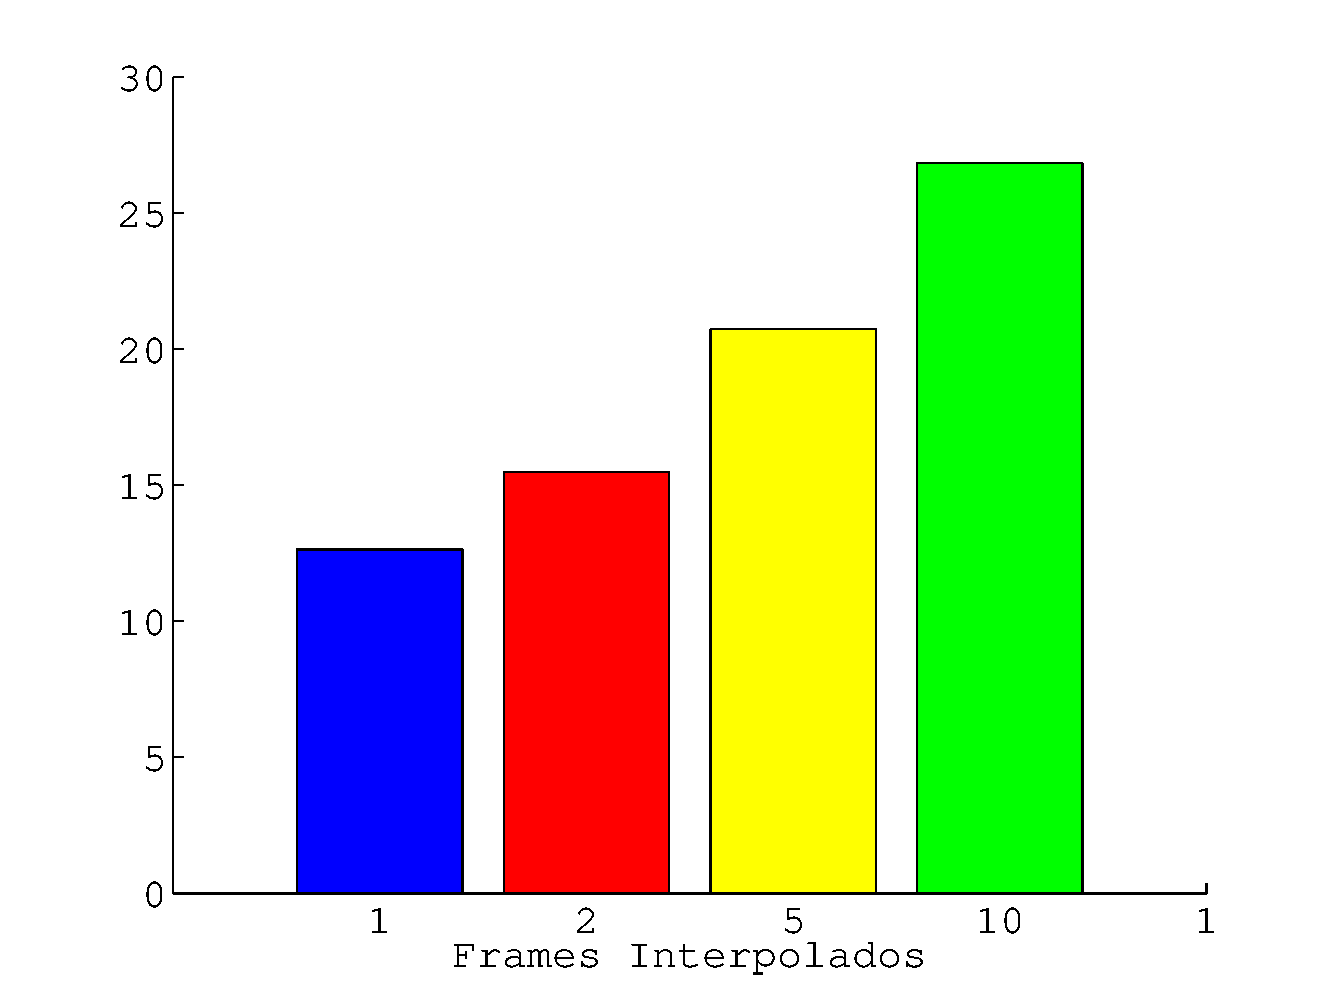
\includegraphics[width=.25\textwidth]{camara_movil-imagen_fija-mean_lineal.pdf}
    }
    \subfloat[][Desv\'io Est\'andar]{
        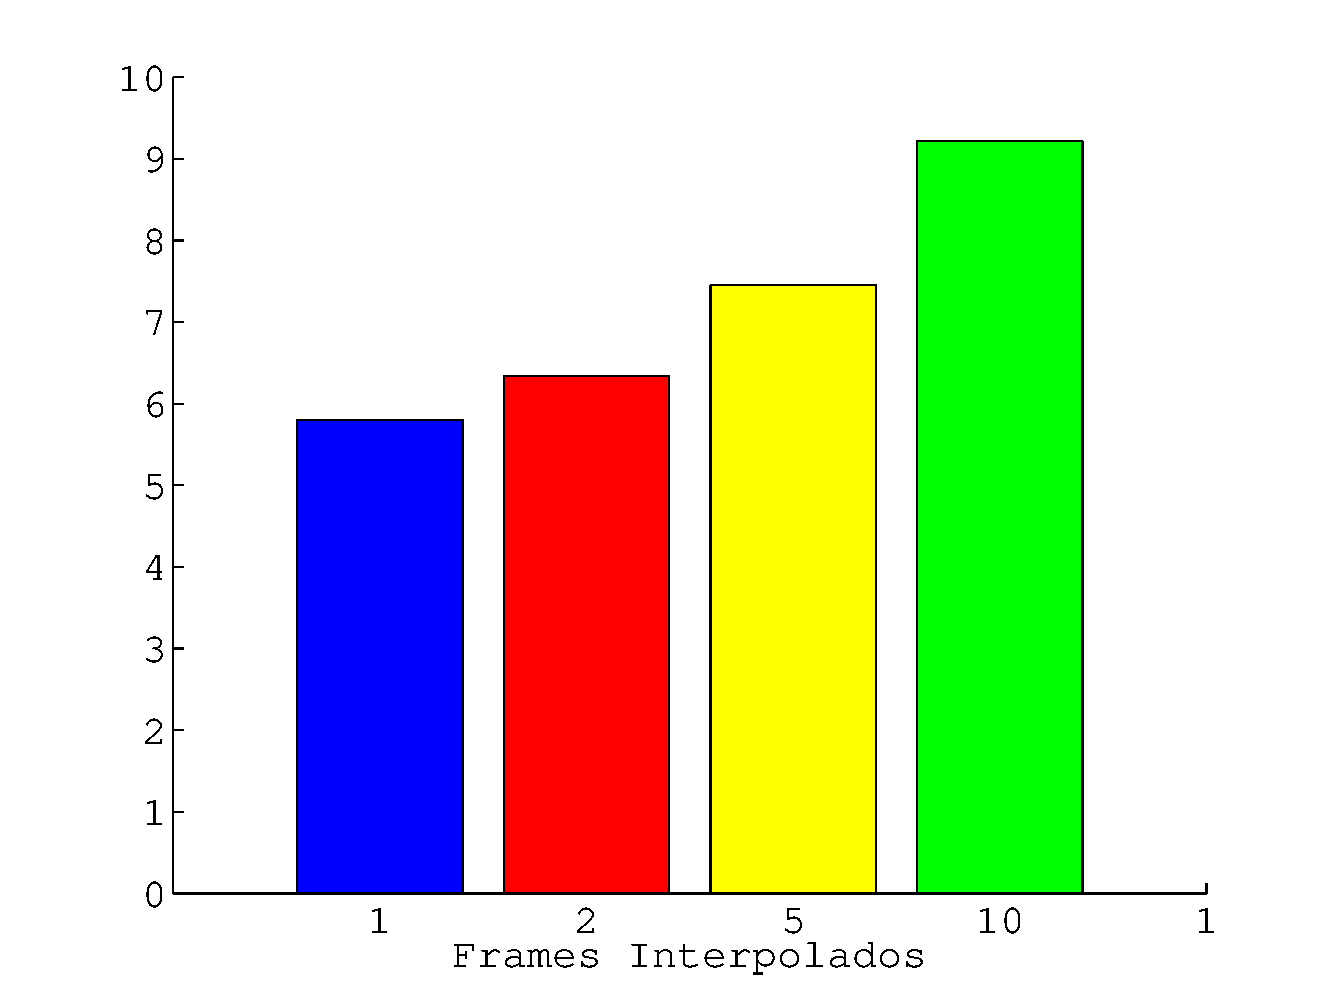
\includegraphics[width=.25\textwidth]{camara_movil-imagen_fija-std_lineal.pdf}
    }
    \subfloat[][M\'aximo]{
        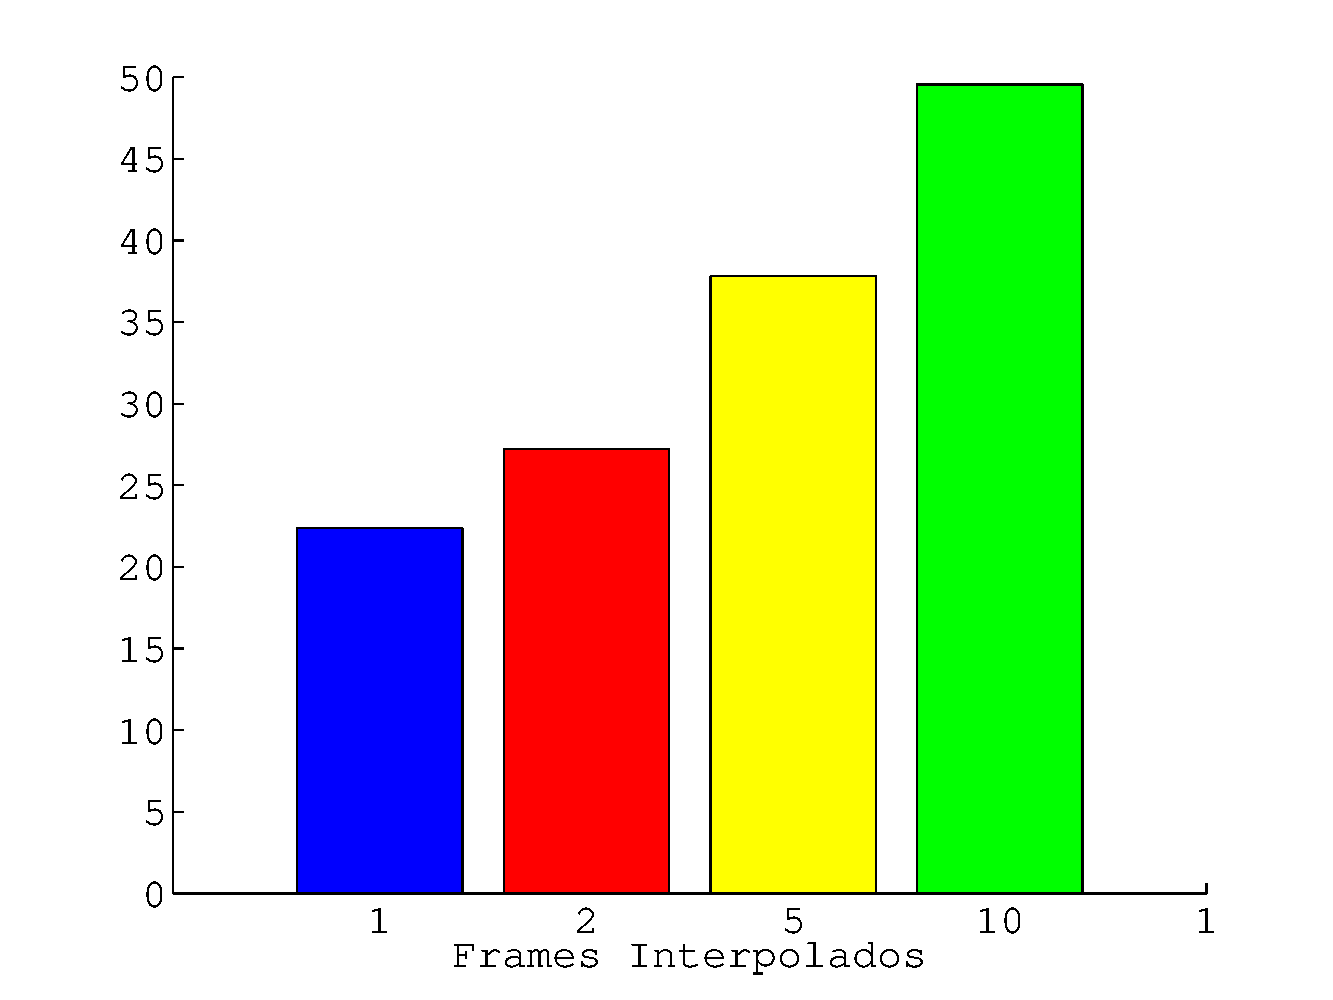
\includegraphics[width=.25\textwidth]{camara_movil-imagen_fija-max_lineal.pdf}
    }
    \subfloat[][M\'inimo]{
        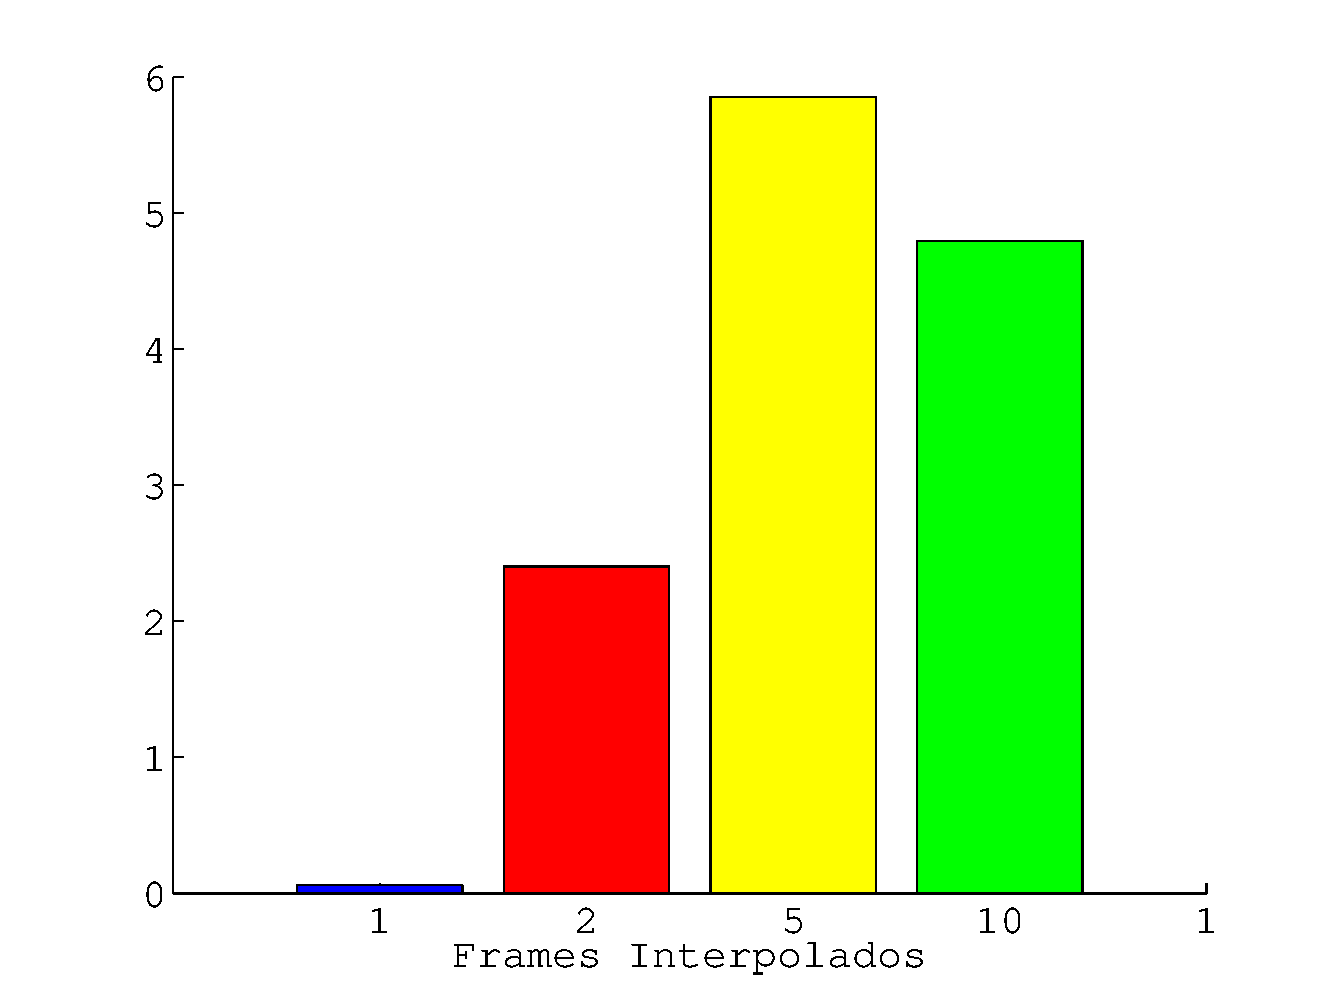
\includegraphics[width=.25\textwidth]{camara_movil-imagen_fija-min_lineal.pdf}
    }
    \caption{Est\'adisticas ECM Seg\'un Frames Interpolados - M\'etodo Lineal}
    \label{fig:movil-fija_lineal-mse_estadisticas}
\end{figure}

\par Aqu\'i los resultados obtenidos son muy similares, en cuanto a la relaci\'on
de las disintas variantes del m\'etodo y no de sus valores nominales, al del
experimento anterior. Nuevamente se observan resultados consistentes con las
hip\'otesis, viendo que el valor medio del error se incrementa a medida que
se deben interpolar m\'as frames, comportamiento que tambi\'en se da para con
el desv\'io est\'andar y el m\'aximo error cometido.

\par En el caso del m\'inimo error cometido, observamos una relaci\'on entre
la variante de 5 frames interpolados y el resto equivalente a la que se vi\'o
para el caso de splines de este mismo experimento. Nuevamente, se intuye que
en el caso de 5 frames existe alg\'un frame utilizado que hace que el m\'etodo
interpole de una manera que pierde una mejor apr\'oximaci\'on, cosa que no
ocurrir\'ia con el caso de 10 frames (la misma hip\'otesis que en el caso
anterior, tener m\'as frames no necesariamente asegura una mejor cota inferior
del error). Por las limitantes de tiempo, no se pudo ahondar m\'as en este
aspecto y buscar comprobar esta hip\'otesis o verificar que otra cosa podr\'ia
estar ocurriendo.

\par Por \'ultimo, al trabajar sobre el video comparativo para 10 frames
interpolados\footnote{\url{https://drive.google.com/open?id=0B0RfkWV-4-XqTy1Ga0F3c09OLVU}},
no vemos diferencia alguna notoria para con el video comparativo de splines
para este experimento, respecto de las regiones/movimientos/caracter\'isticas
que m\'as afectan a la estimaci\'on del frame. Nuevamente, aquellas regiones
regiones que presentan movimiento son aquellas que m\'as afectan al error.

\par De la observaci\'on de este video, se observ\'o una nueva caracter\'istica
que tambi\'en aplica al caso de splines: las partes de la figura que est\'a
siendo observada circularmente por la c\'amara que m\'as aportan al error
tienden a ser las partes m\'as cercanas al contorno de la figura. Entendemos
que esto ocurre por 2 motivos, el primero es que la figura est\'a est\'atica y
debido al movimiento de la c\'amara, siempre est\'a en el centro del (es decir,
la regi\'on del frame que presenta el movimiento/cambios siempre es un primer
plano centrado de los cuadros). El segundo hecho es que la figura suele ser del
mismo color o tonalidades del mismo. As\'i pues, al rotar la c\'amara y los
p\'ixeles ''desplazarse''\footnote{En realidad ocurre que la representaci\'on
de un pixel de un frame a otro cambia de pixel, pero la sensaci\'on para el que
mira el video es la explicada.} pasan a ocupar un lugar que en el frame previo
era seguramente de un color/tonalidad similar, lo cual hace que el m\'etodo
cometa un error menor.  Esto \'ultimo no se dar\'ia en los contornos de la
figura, donde un pixel pasa de representar a alguna parte de la figura en un
frame, y en el siguiente representa una parte del fondo de la im\'agen,
teniendo un cambio m\'as abrupto de color/tonalidad y por lo tanto haciendo que
el m\'etodo comenta m\'as error (ya que la interpolaci\'on trata de aproximar a
una supuesta funci\'on ''suave''\footnote{Definimos \emph{suave} como que para
valores de $x$ inmediatos o muy cercanos, el valor de $f(x)$ tambi\'en es muy
cercano.}).

\par En la figura \ref{fig:movil-fija_lineal-heatmap-contornos} se observa una
captura representativa de este comportamiento, observable en el video
comparativo. En el mismo queda claro que la interpolaci\'on comete mucho m\'as
error en los contornos/relieves de la figura que en las partes
planas\footnote{Refiri\'endonos a la tonalidad de la figura.}.

\begin{figure}[H]
    \centering
    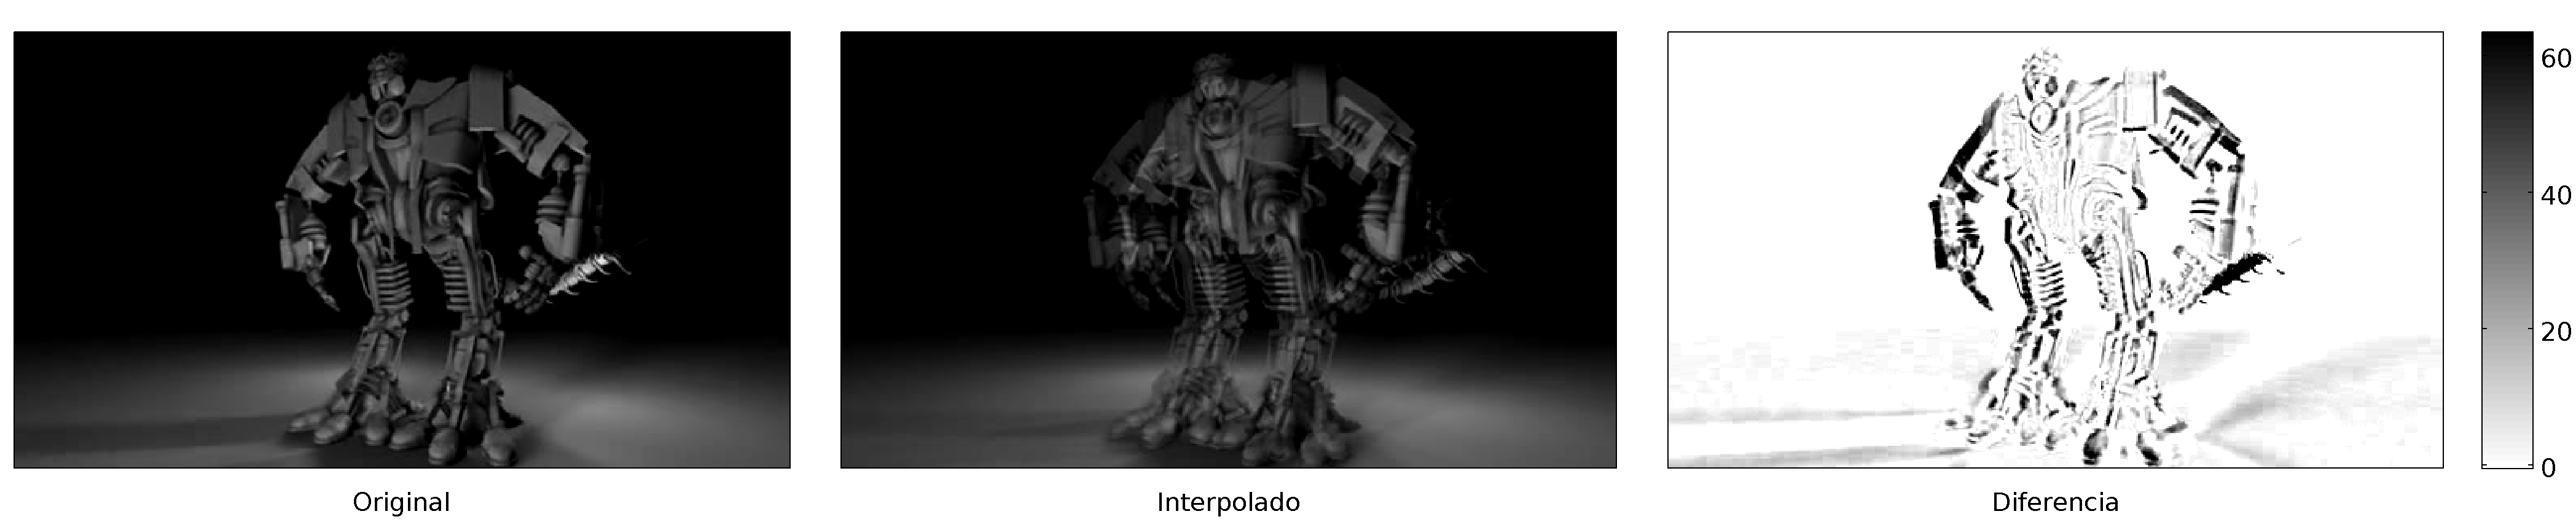
\includegraphics[width=\textwidth]{camara_movil-imagen_fija-lineal-k10-contornos.png}
    \label{fig:movil-fija_lineal-heatmap-contornos}
    \caption{Mayor error en los contornos de la Figura est\'atica}
\end{figure}

%---------------------------------------------------------------
\subsubsection{Vecino m\'as Cercano}

\begin{figure}[H]
    \centering
    \subfloat[][Valor Medio]{
        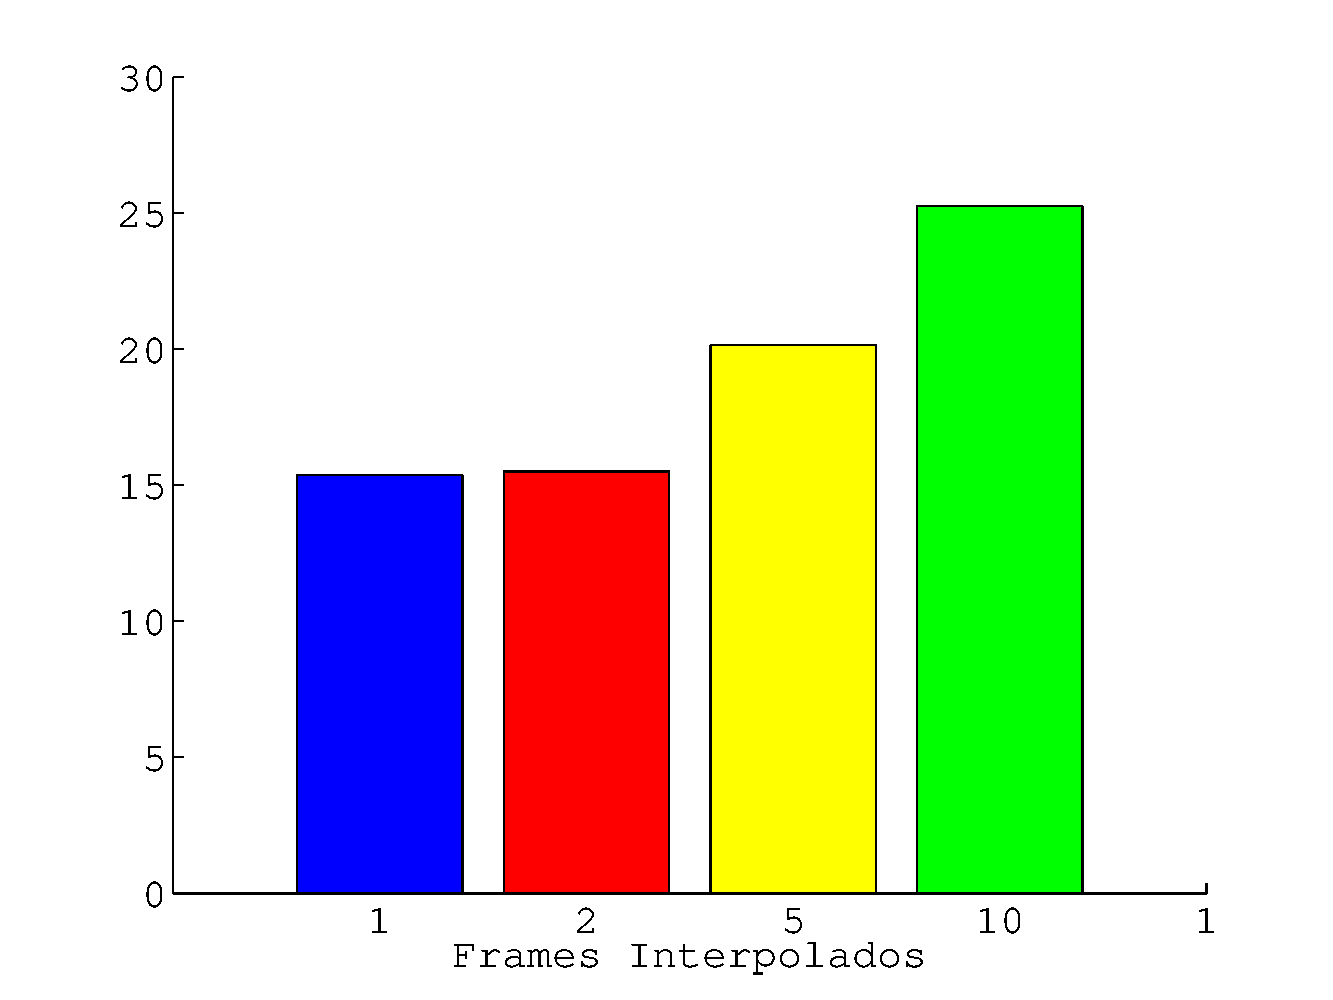
\includegraphics[width=.25\textwidth]{camara_movil-imagen_fija-mean_vecino.pdf}
    }
    \subfloat[][Desv\'io Est\'andar]{
        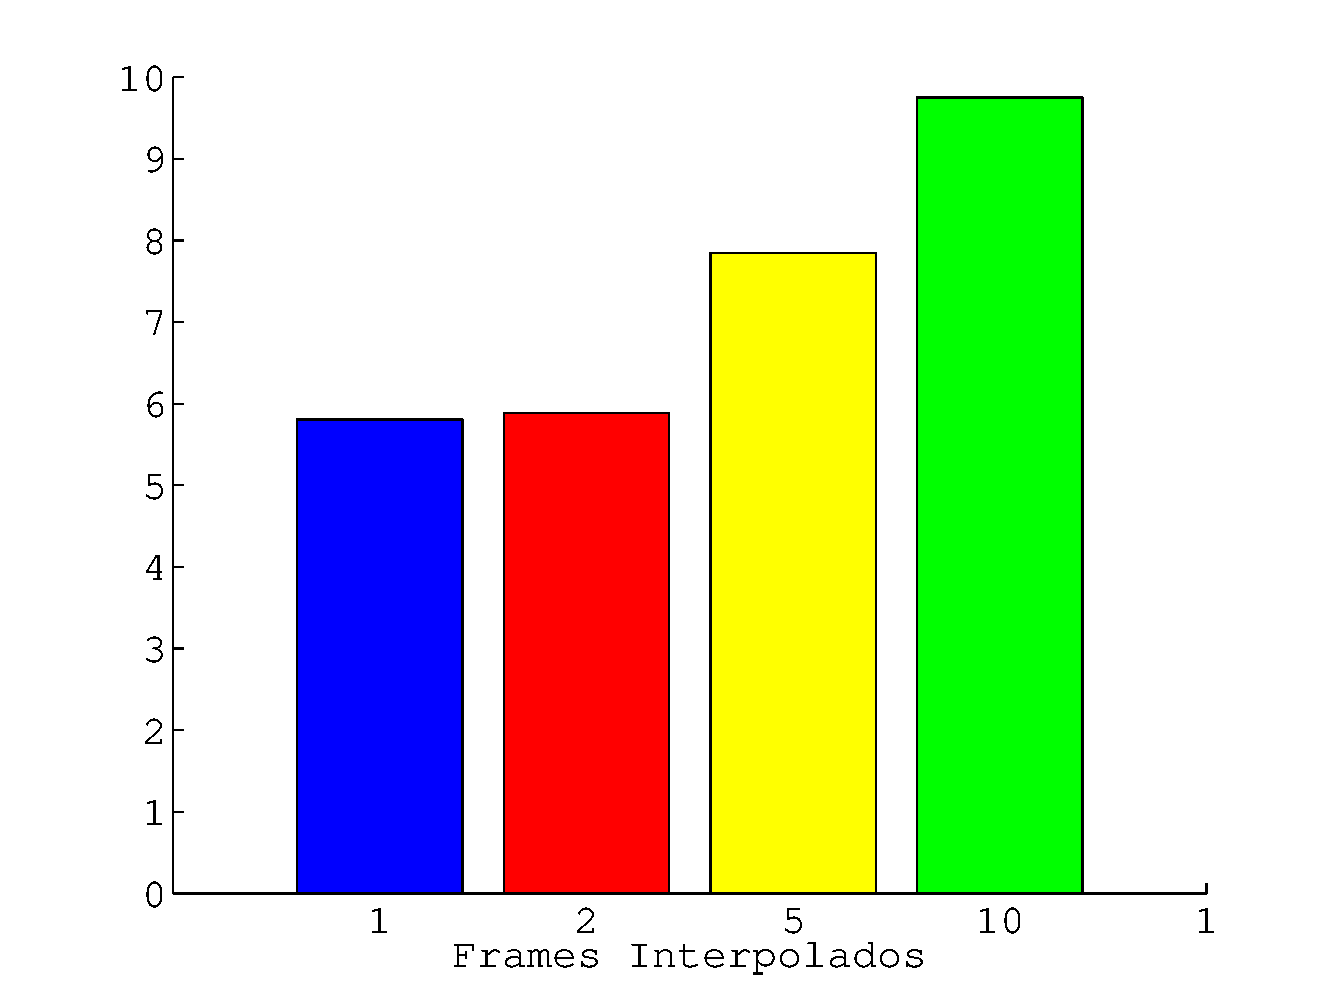
\includegraphics[width=.25\textwidth]{camara_movil-imagen_fija-std_vecino.pdf}
    }
    \subfloat[][M\'aximo]{
        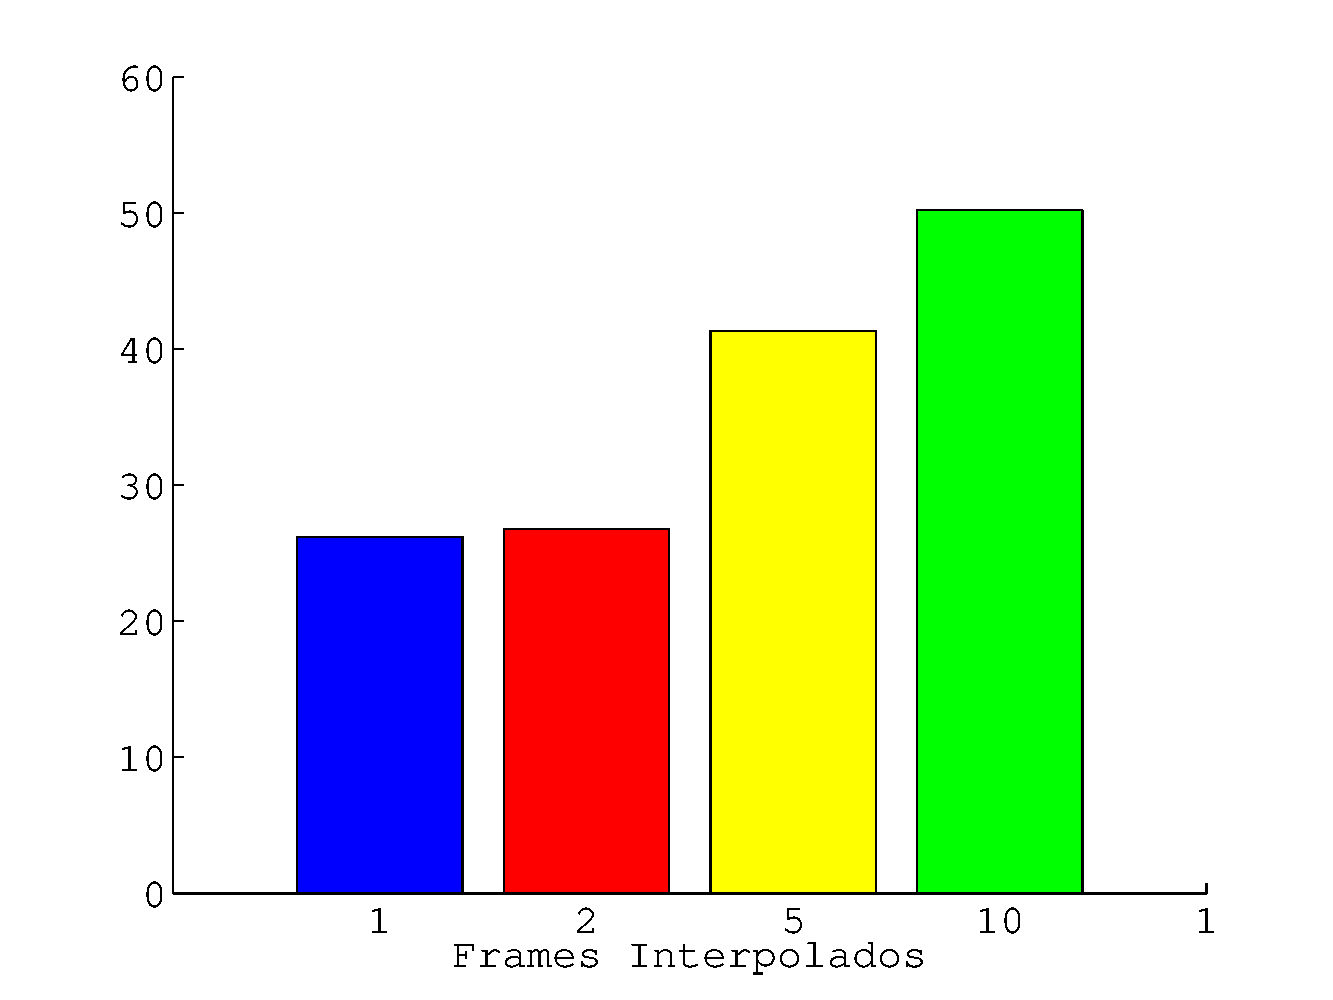
\includegraphics[width=.25\textwidth]{camara_movil-imagen_fija-max_vecino.pdf}
    }
    \subfloat[][M\'inimo]{
        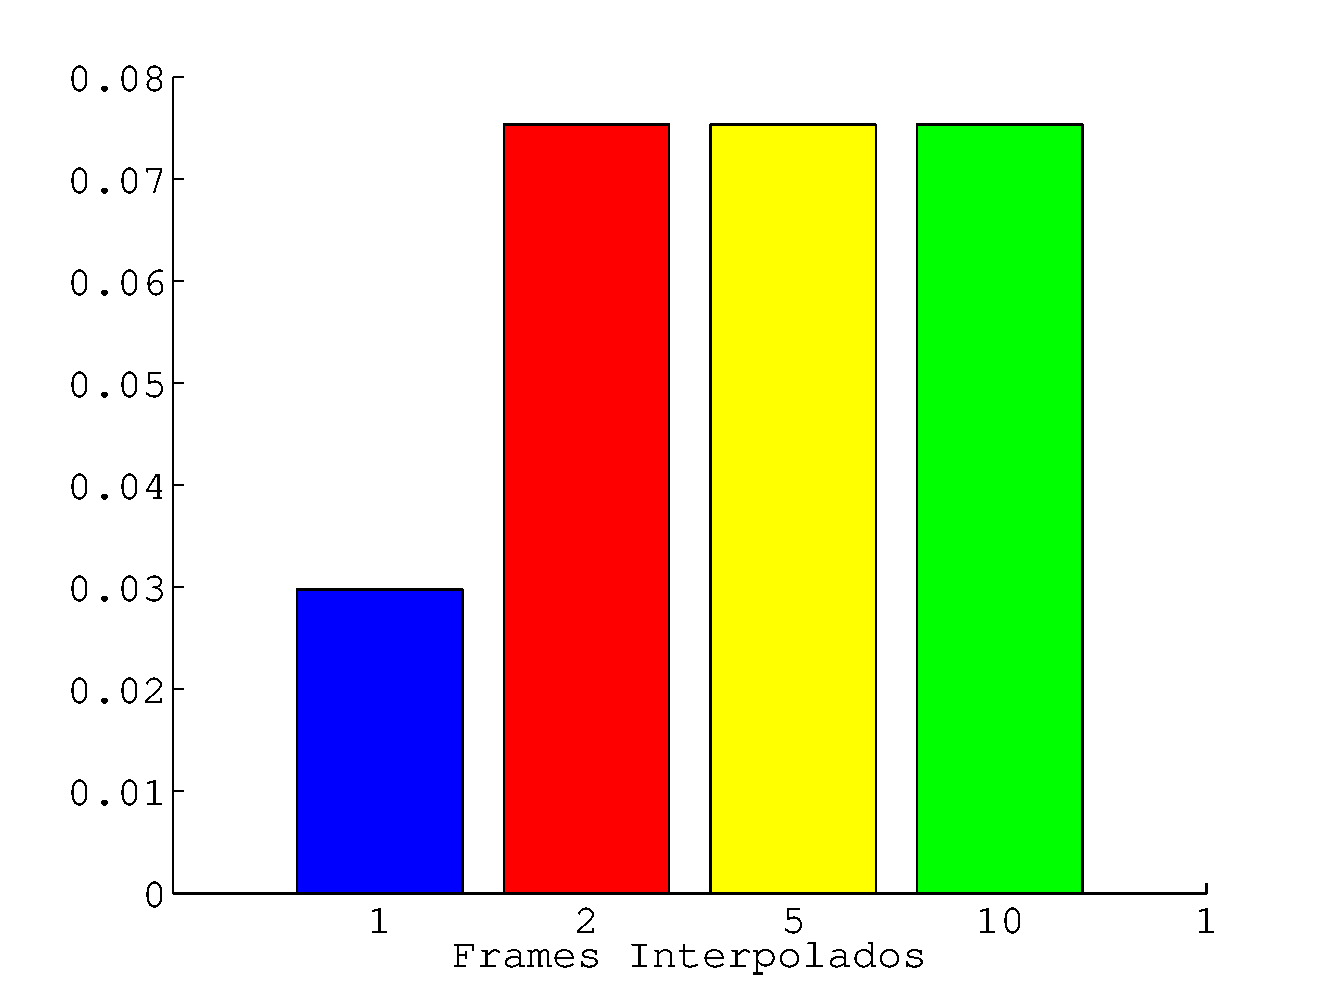
\includegraphics[width=.25\textwidth]{camara_movil-imagen_fija-min_vecino.pdf}
    }
    \caption{Est\'adisticas ECM Seg\'un Frames Interpolados - M\'etodo Lineal}
    \label{fig:movil-fija_vecino-mse_estadisticas}
\end{figure}

\par Los resultados obtenidos no distan de las hip\'otesis planteadas. La media
del ECM se incrementa a mayor cantidad de frames, como as\'i lo hace su error
m\'aximo y desv\'io est\'andar. Esto tiene sentido, como incluso se a explicado
en el experimento previo, ya que al tener cada vez m\'as frames, habr\'a cada
vez m\'as frames copiados que estar\'an m\'as alejados del frame original o su
''vecino m\'as cercano'', haciendo que haya m\'as error y m\'as valores alejados
de una media. A su vez, se observa como el error m\'inimo alcanzado es menor
para para la interpolaci\'on de 1 frame, lo cual no es conciso respecto de
nuestras hip\'otesis. Aunque si se presta atenci\'on a la escala del error, se
ver\'a que la diferencia es menor a $0,05$, lo cual es un valor claramente muy
peque\~no e indistinguible al ojo humano (por lo cual se podr\'ia llegar a
considerar que en realidad el error m\'inimo es el mismo para todos las
variantes).

\par El motivo de esta diferencia se debe al m\'etodo de ''desempate'' de la
implementaci\'on del m\'etodo. Al interpolar de a un \'unico frame entre 2,
se toma el frame mayor\footnote{Aquel que se reproduce m\'as tarde.}, y se
da en el caso particular de este video que interpolar con vecino m\'as cercano
el frame n\'umero 2 copiando el frame n\'umero 3 en lugar del n\'umero 1 (lo
que ocurre en las otras variantes) genera un ECM menor. De hecho, esto puede
observarse en los gr\'aficos de la figura \ref{fig:movil-fija_vecino-frames},
donde se que el PSNR mayor (que se corresponde con el ECM menor) se encuentra
en el primer frame interpolado.

\par Otro comportamiento interesante observado es como var\'ia el ECM/PSNR
en funci\'on de la cantidad de frames interpolados. Como ya se ha explicado,
comprara estas m\'etricas frame a frame para dos cualesquiera de estas variantes
no es \'util, ya que los frames interpolados no coincidir\'an necesariamente
(s\'olo algunos pocos lo har\'an). A\'un as\'i, si observamos los gr\'aficos
del PSNR de la figura \ref{fig:movil-fija_vecino-frames} veremos como la calidad
de la aproximaci\'on a los frames originales pasa de ser algo m\'as suave para
pocos frames y comienza a tener cambios bruscos (picos, o comportamiento de
\emph{dientes de sierra}) a medida que se incrementan la cantidad de frames.

\begin{figure}[H]
    \centering
    \subfloat[][1 frame]{
        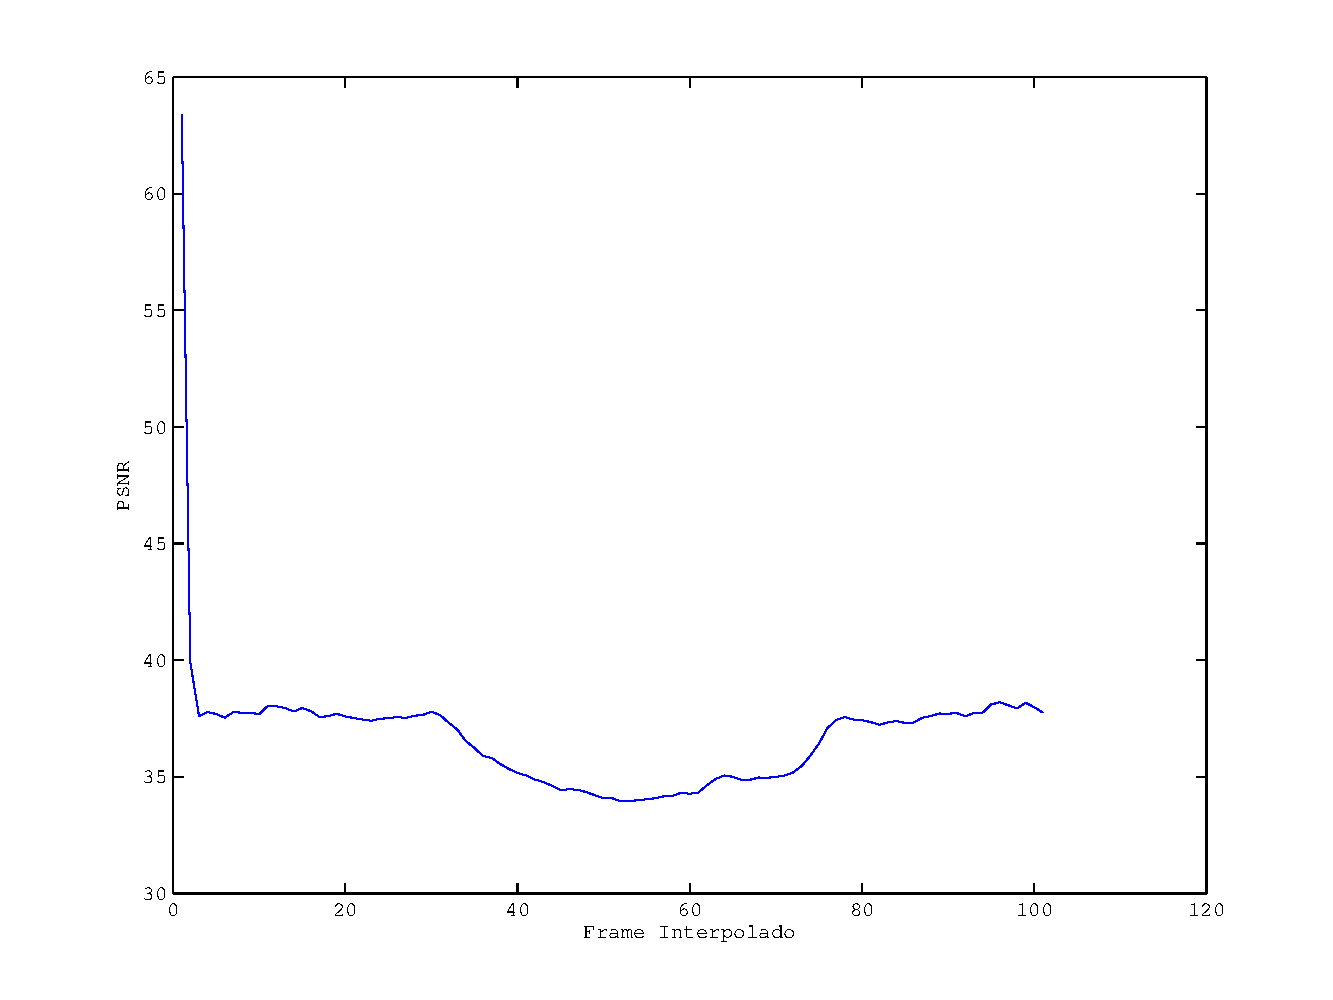
\includegraphics[width=.25\textwidth]{camara_movil-imagen_fija-VECINO-psnr-k1.pdf}
    }
    \subfloat[][2 frames]{
        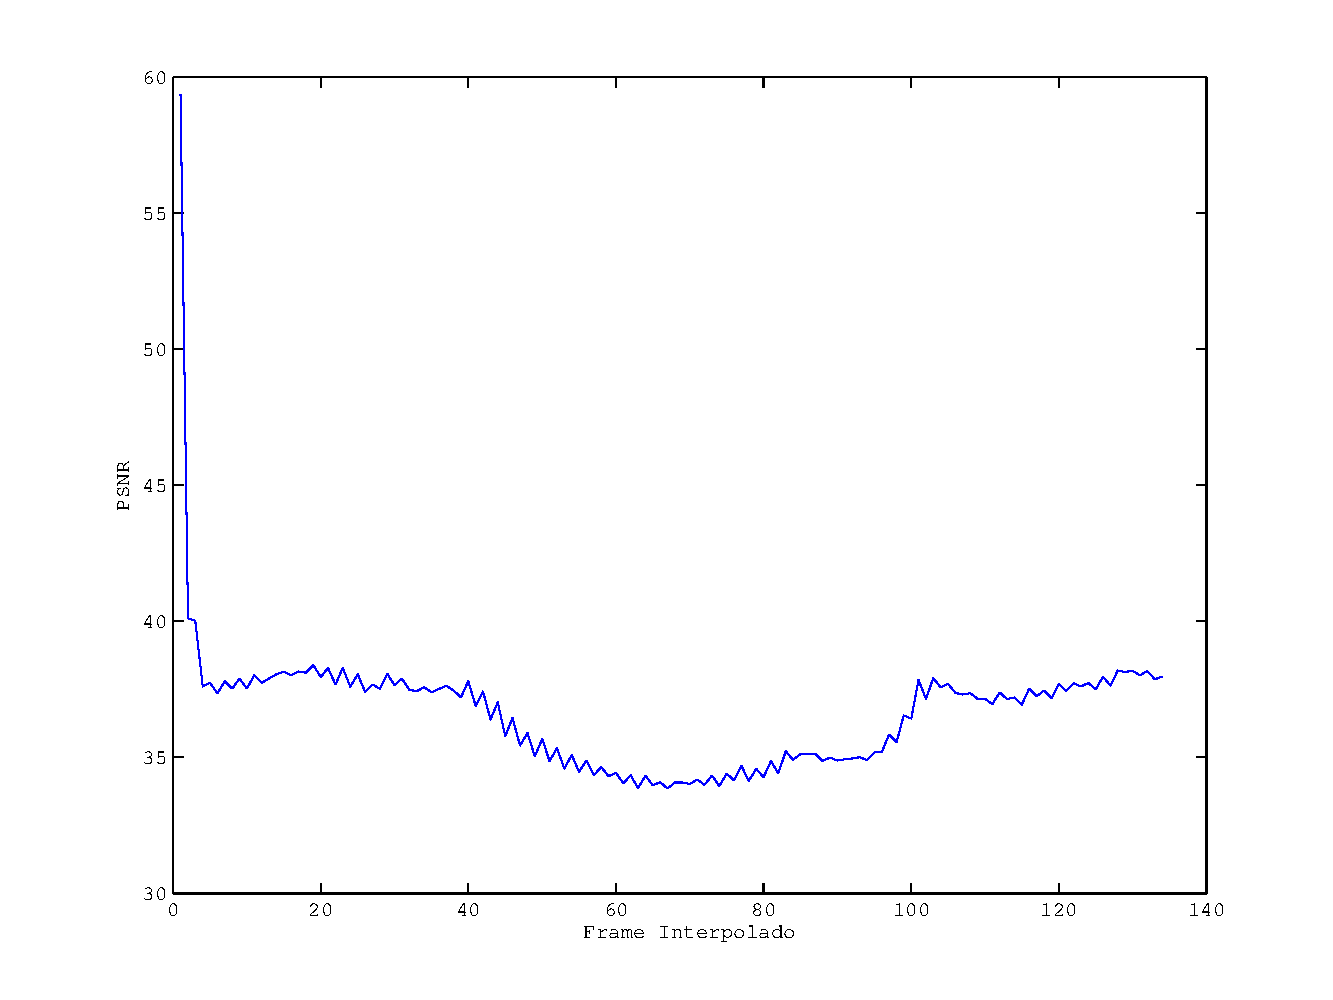
\includegraphics[width=.25\textwidth]{camara_movil-imagen_fija-VECINO-psnr-k2.pdf}
    }
    \subfloat[][5 frames]{
        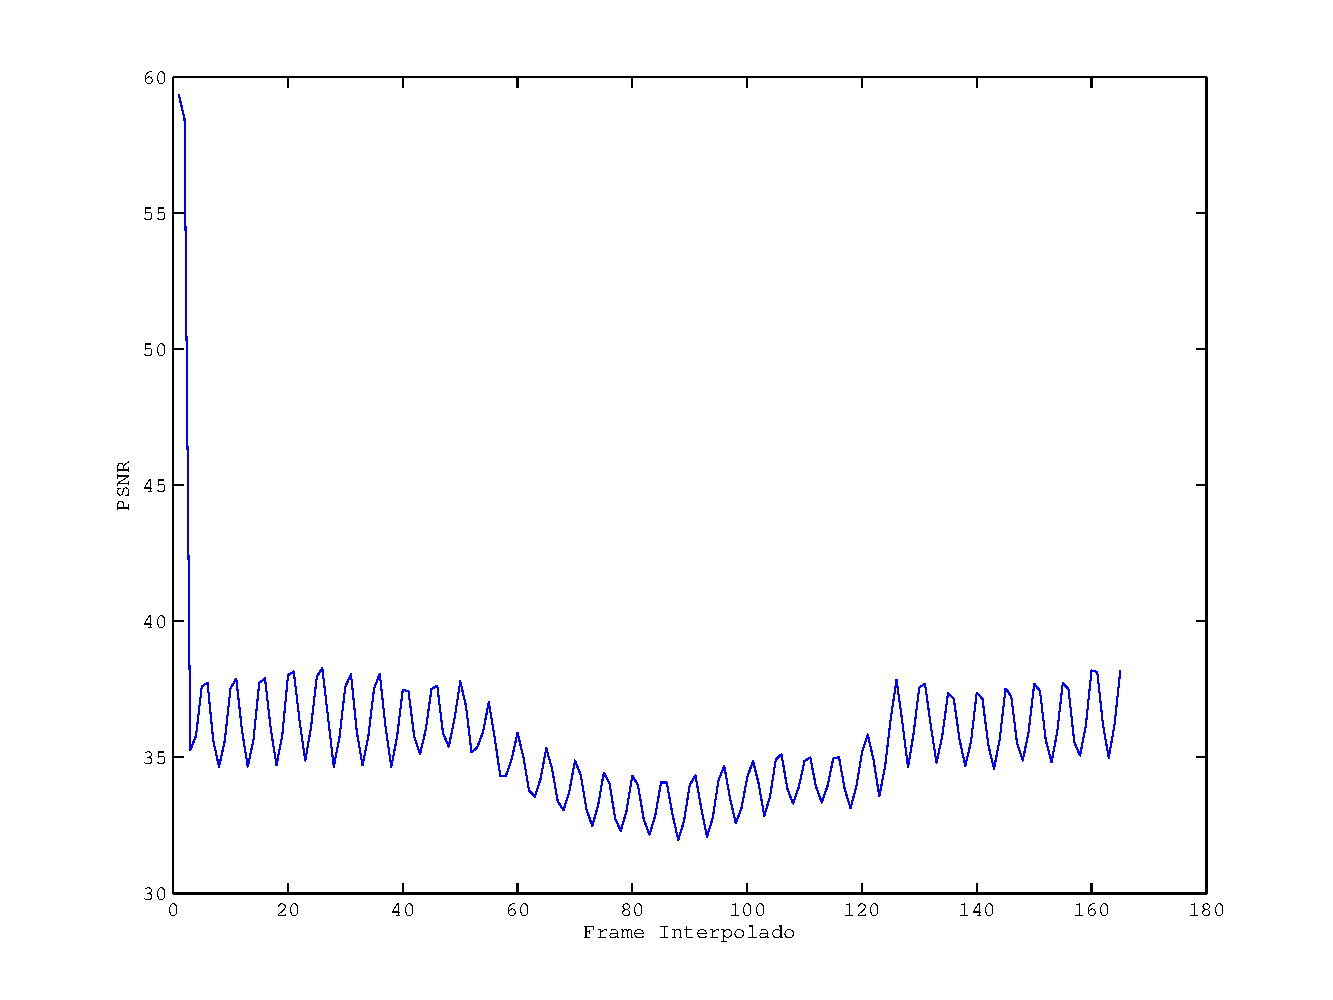
\includegraphics[width=.25\textwidth]{camara_movil-imagen_fija-VECINO-psnr-k5.pdf}
    }
    \subfloat[][10 frames]{
        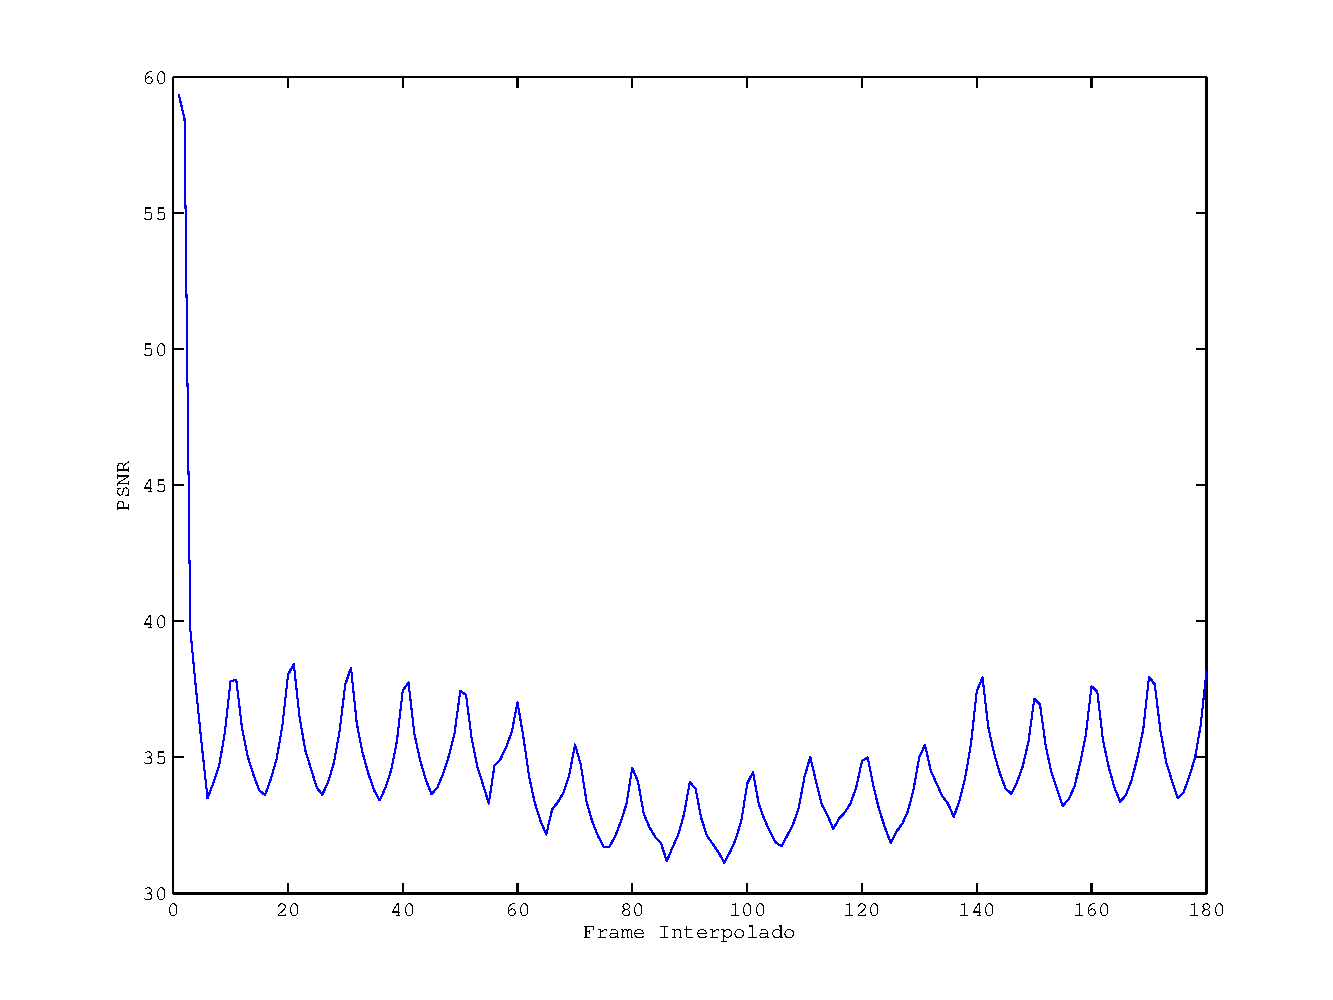
\includegraphics[width=.25\textwidth]{camara_movil-imagen_fija-VECINO-psnr-k10.pdf}
    }
    \caption{PSNR en funci\'on de cantidad de frames interpolados - M\'etodo lineal}
    \label{fig:movil-fija_vecino-frames}
\end{figure}

\par Esto se debe a la distancia de una copia/frame interpolado respecto del
frame original. A medida que el frame interpolado est\'a m\'as cerca del frame
original (es decir, en el orden de reproducci\'on est\'a a menor distancia de
aquel que fue copiado), menor ser\'a el error y mayor el PSNR (los picos altos),
y al inversamente, al alejarse del frame original su error se incrementar\'a
y su PSNR bajar\'a (los picos bajos).

\par De hecho, este comportamiento se ve de forma muy clara en el video
video comparador para 10 frames
interpolados\footnote{\url{https://drive.google.com/open?id=0B0RfkWV-4-XqYWRfaG8xdlNscWs}}.
En el mismo se observa como a medida que avanza la reproducci\'on, las
diferencias con el frame interpolado van aumentando hasta llegar un punto en
que se cambi\'a el frame (pasamos al vecino m\'as cercano del siguiente frame
original) y la diferencia con el frame original comienza a ir cada vez siendo
menor (y luego comienza de vuelta este ciclo).

\par Justamente esto es consistente con la m\'etrica del desv\'io estandar
expuesto m\'as arriba. Al tener m\'as frames interpolados, tendremos un
comportamiento de ''diente de sierra'' m\'as marcado y por lo tanto los valores
del error estar\'an cada vez a distancias m\'as variables respecto de la media.

%---------------------------------------------------------------
\subsubsection{An\'alisis entre M\'etodos}
\par A continuaci\'on comparamos los distintos m\'etodos entre s\'i. En el caso
de splines, se decidi\'o usar los resultados para el tama\~no de bloque
equivalente al tama\~no del video (es decir, un \'unico bloque), ya que se
vi\'o previamente que el tama\~no de bloque no influ\'ia siginficativamente
en los resultados.

\begin{figure}[H]
    \centering
    \subfloat[][ECM para 1 frames interpolados]{
        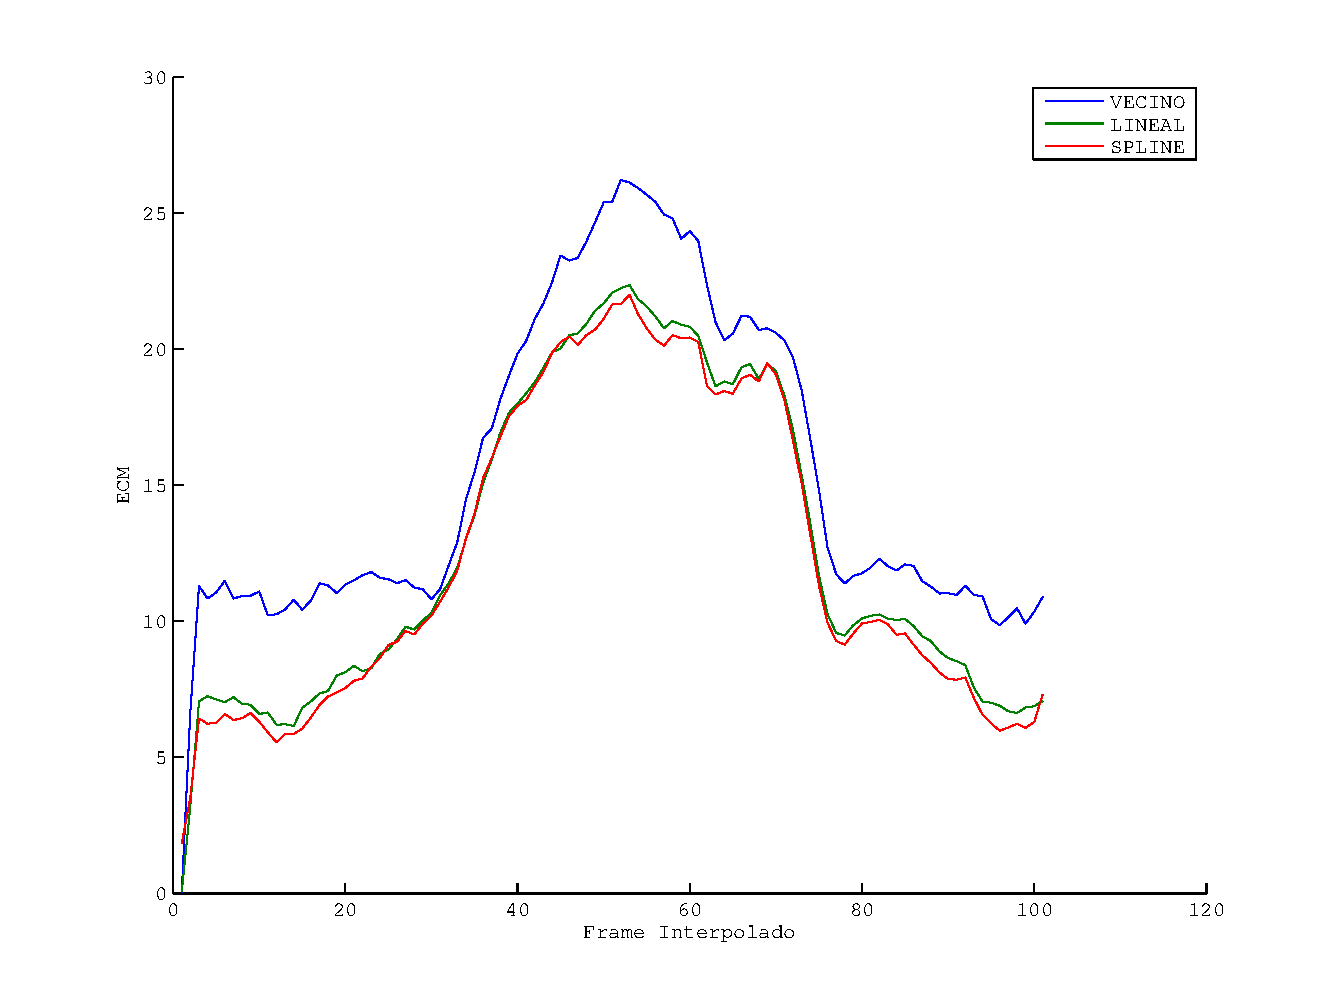
\includegraphics[width=.5\textwidth]{mse_methods-camara_movil-imagen_fija-k1.pdf}
        \label{subfig:movil-fija_mse-k1}
    }
    \subfloat[][ECM para 2 frames interpolados]{
        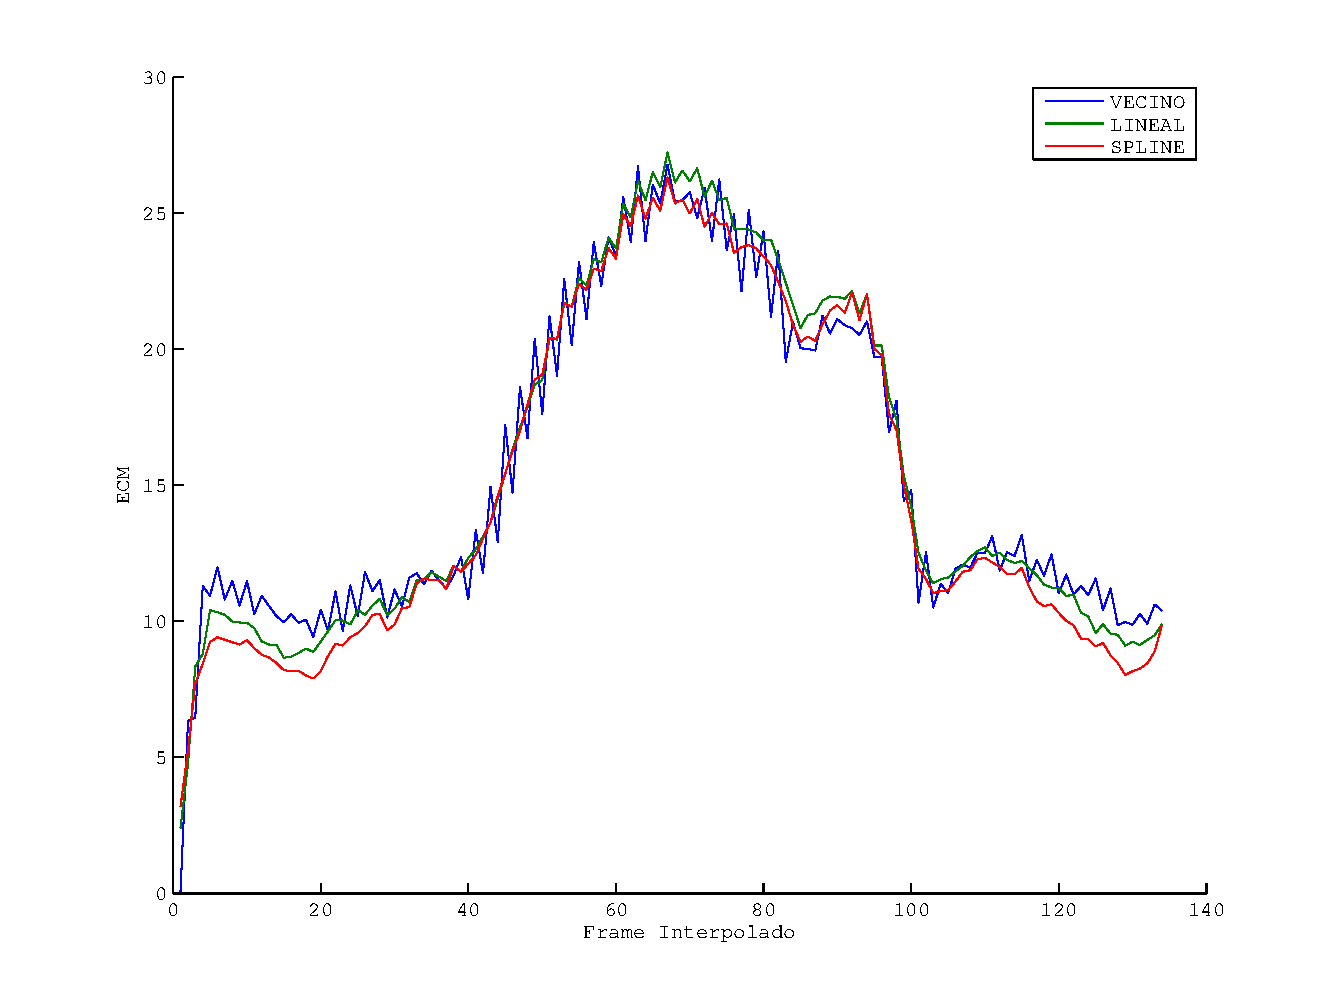
\includegraphics[width=.5\textwidth]{mse_methods-camara_movil-imagen_fija-k2.pdf}
        \label{subfig:movil-fija_mse-k2}
    }\\
    \subfloat[][ECM para 5 frames interpolados]{
        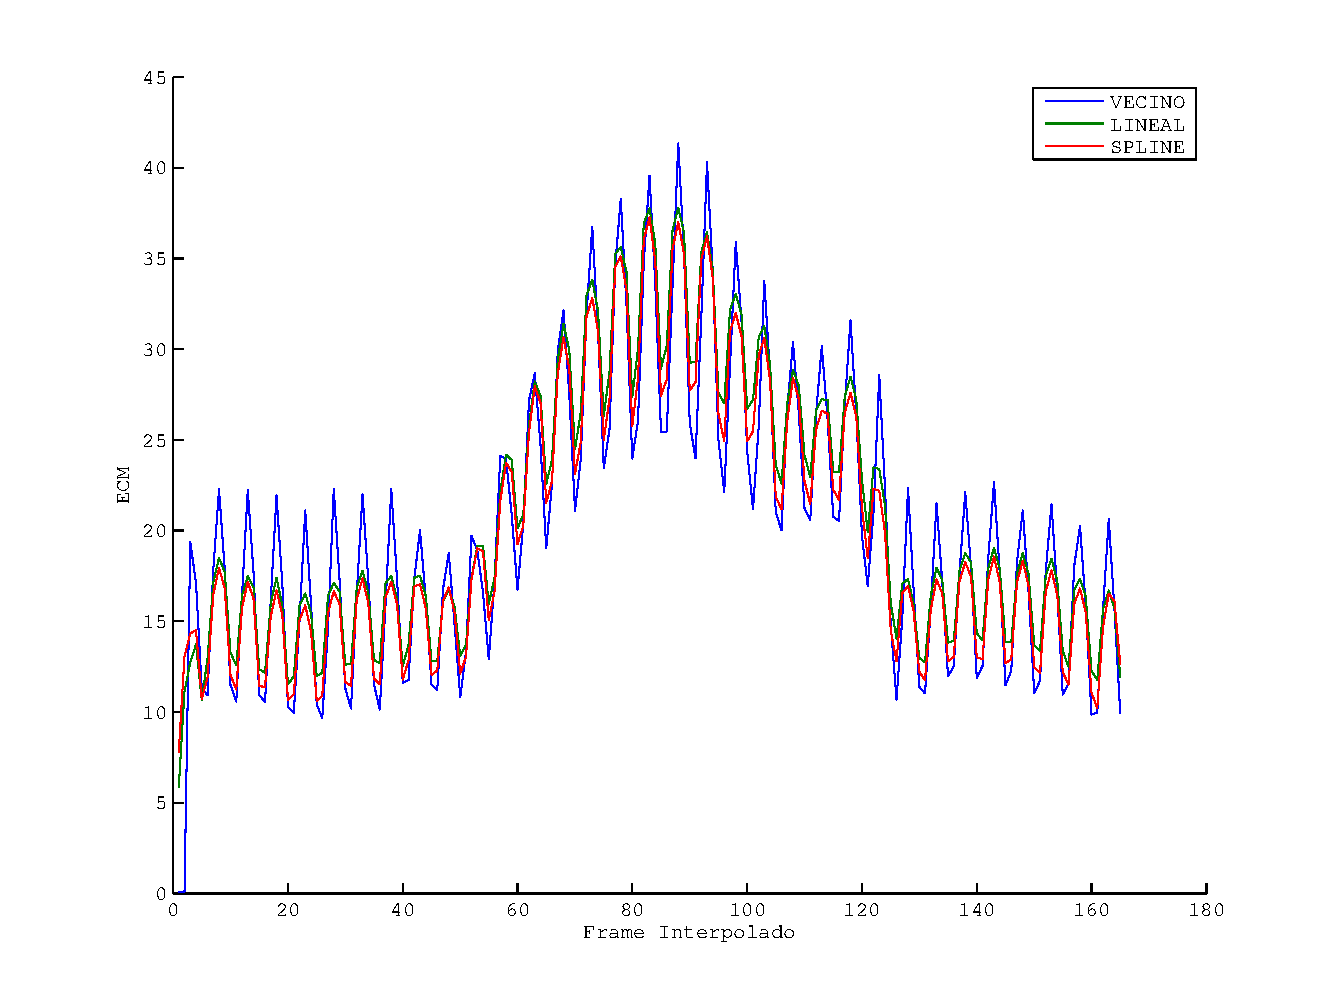
\includegraphics[width=.5\textwidth]{mse_methods-camara_movil-imagen_fija-k5.pdf}
        \label{subfig:movil-fija_mse-k5}
    }
    \subfloat[][ECM para 10 frames interpolados]{
        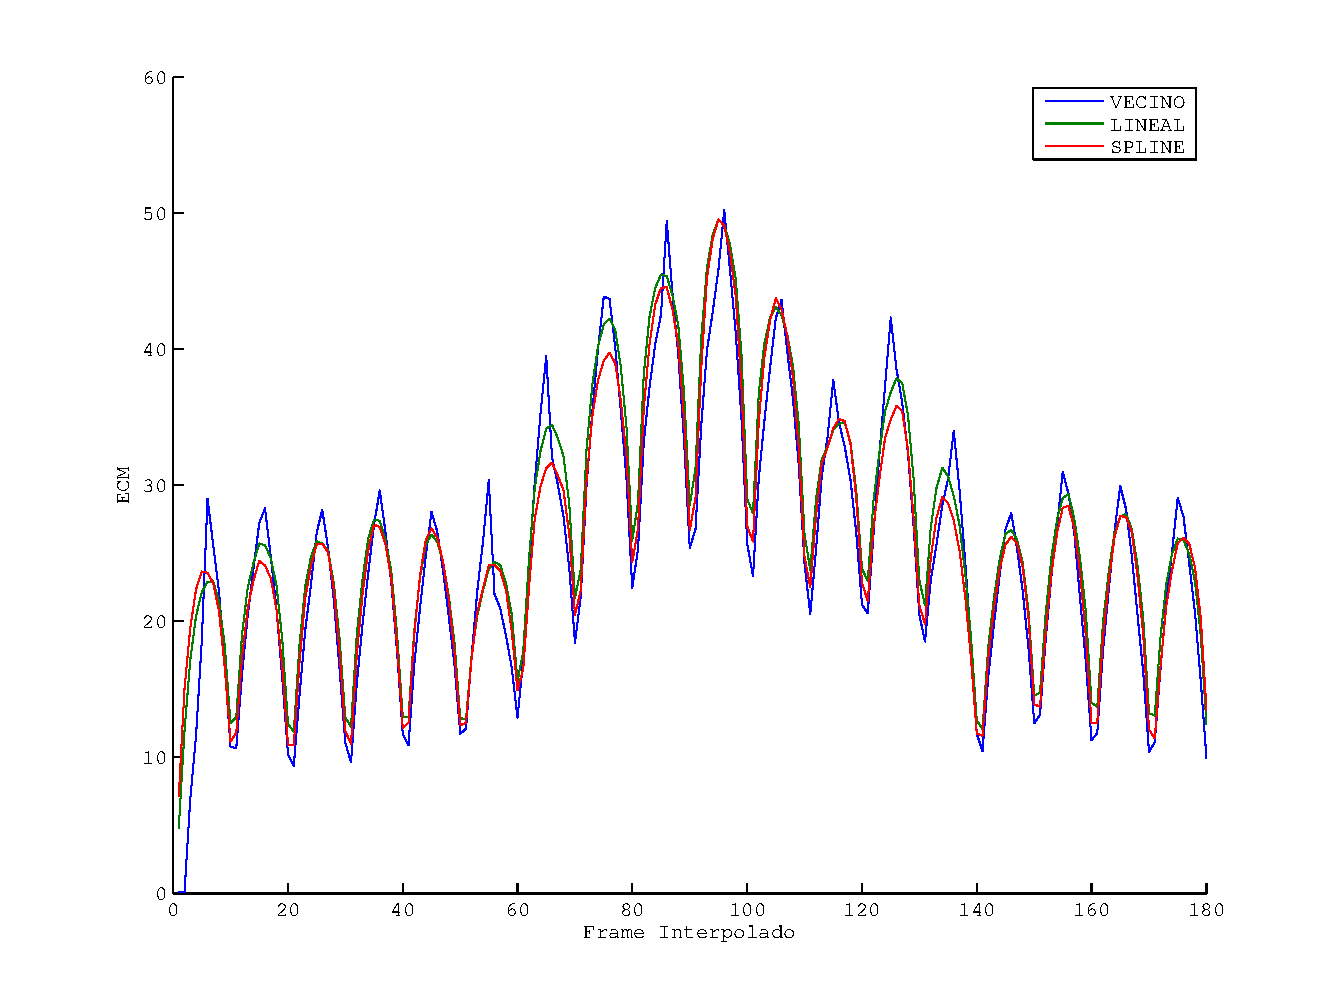
\includegraphics[width=.5\textwidth]{mse_methods-camara_movil-imagen_fija-k10.pdf}
        \label{subfig:movil-fija_mse-k10}
    }
    \caption{Comparativa de m\'etodos}
    \label{fig:movil-fija_metodos}
\end{figure}

\par Lo que se observa en la figura \ref{fig:movil-fija_metodos} nos muestra que
a menor cantidad de frames interpolados, la diferencia entre el error de los
m\'etodos es m\'as clara, y a medida que se interpolan m\'as frames comienza
a ser notoriamente m\'as dificil distinguir quien comete m\'as errores (de hecho,
ya es dif\'icil determinar esto para 2 frames interpolados, aunque es posible
mirando con mucha atenci\'on la figura \ref{subfig:movil-fija_mse-k2}).

\par Otro comportamiento que se puede determinar es que a medida que se
interpolan m\'as frames, todos los m\'etodos comienzar a oscilar entre valores
altos y bajos de error (aunque vecino m\'as cercano comienza a oscilar ya para
2 frames interpolados). En esta l\'inea, tambi\'en se observa que los picos de
error (tanto altos como bajos) del m\'etodo del vecino son mayores y menores
que los picos de los restantes m\'etodos. Se podr\'ia decir, coloquialmente,
que el m\'etodo del vecino oscila de manera m\'as brusca y amplia que sus
contrapartes.

\par Una \'ultima observaci\'on a realizar antes de pasar a los datos
est\'adisticos del ECM es que, m\'as all\'a de los solapamientos y algunas
secuencias de frames, el m\'etodo de spline pareciera comenzar a ganar terreno
sobre del error comentido respecto de interpolaci\'on lineal y vecino a medida
que se interpolan m\'as frames. De hecho, esto se confirma con los valores
presentados en la figura \ref{fig:movil-fija_methods-mse_estadisticas}.

\begin{figure}[H]
    \centering
    \subfloat[][Valor Medio]{
        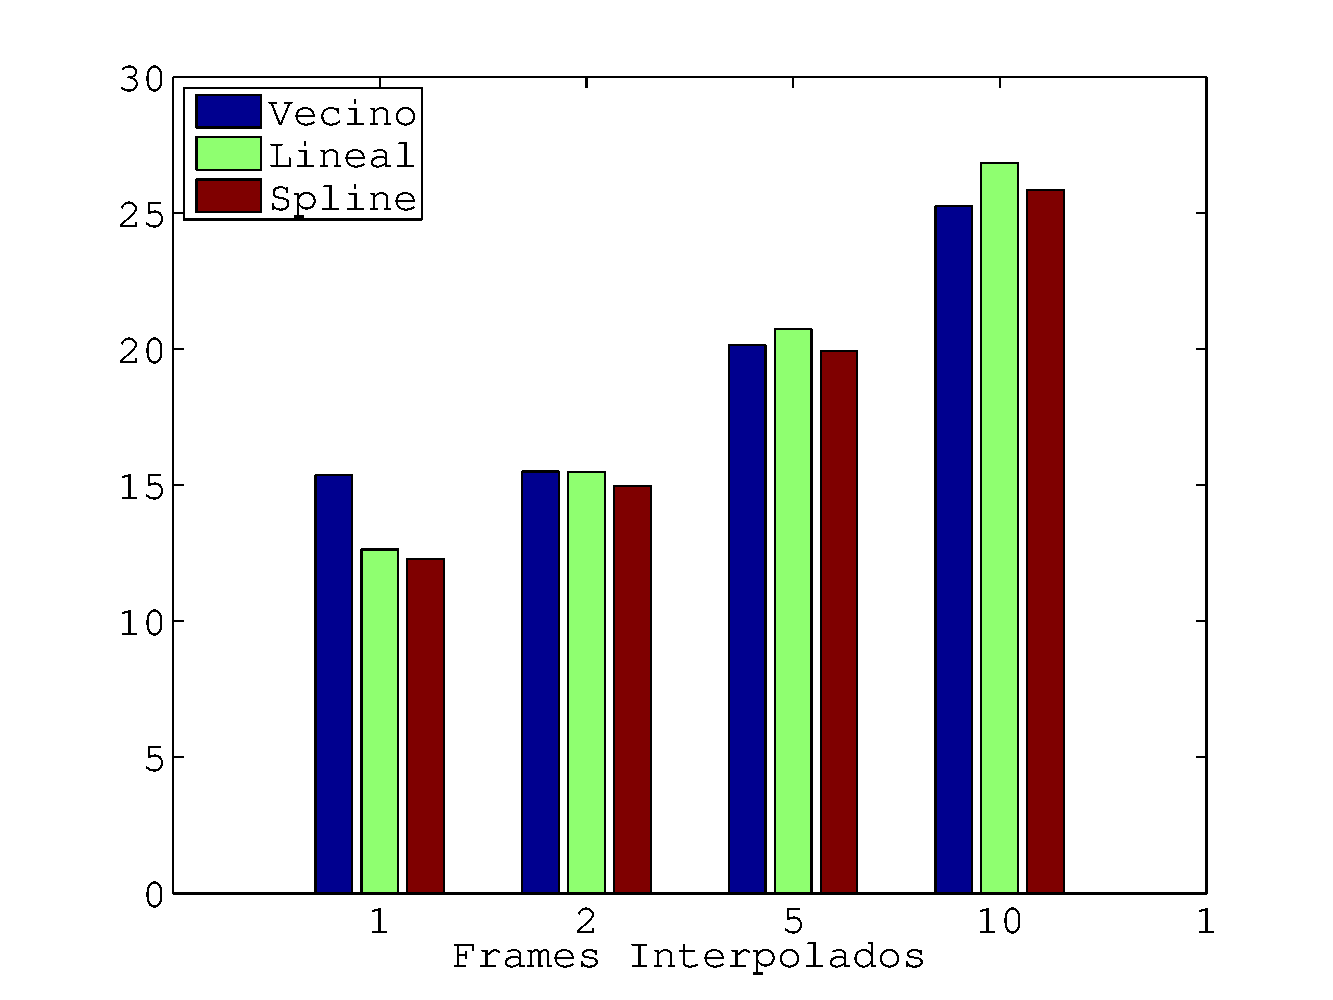
\includegraphics[width=.5\textwidth]{mean_methods-camara_movil-imagen_fija.pdf}
    }
    \subfloat[][Desv\'io Est\'andar]{
        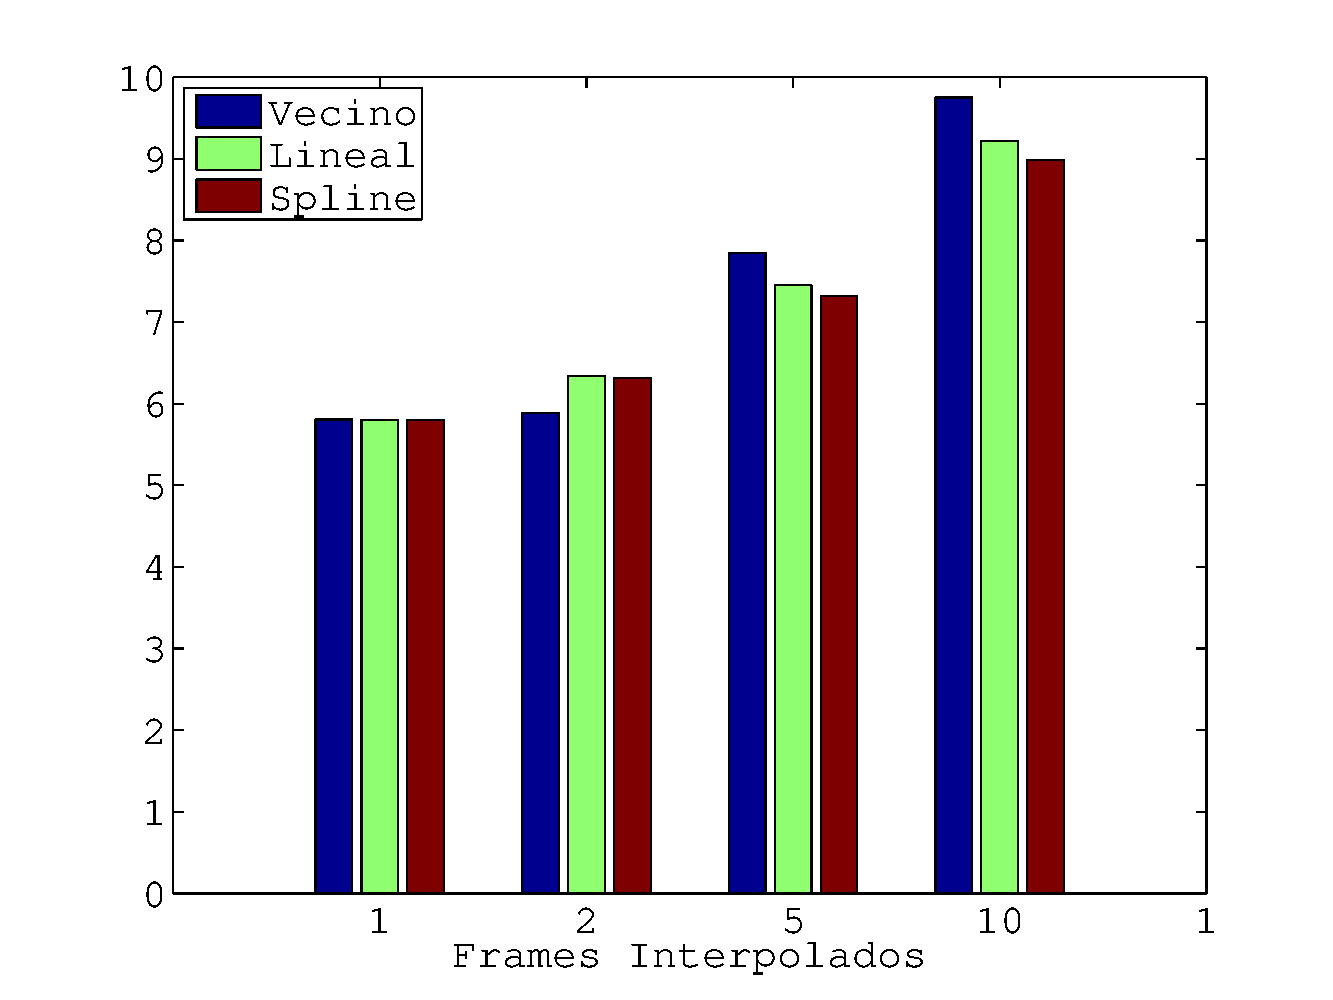
\includegraphics[width=.5\textwidth]{std_methods-camara_movil-imagen_fija.pdf}
    }\\
    \subfloat[][M\'aximo]{
        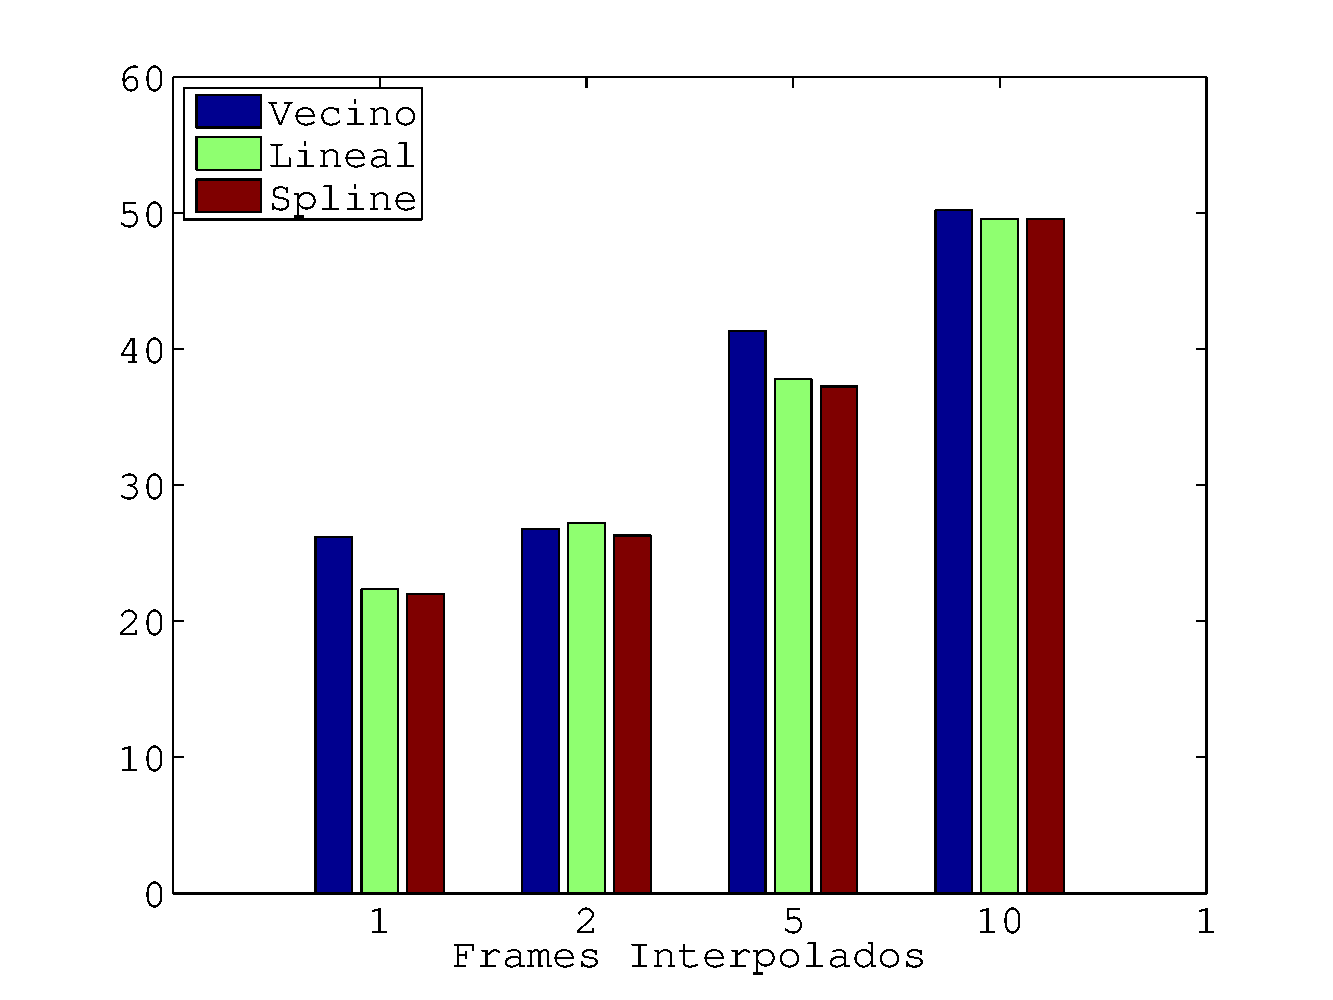
\includegraphics[width=.5\textwidth]{max_methods-camara_movil-imagen_fija.pdf}
    }
    \subfloat[][M\'inimo]{
        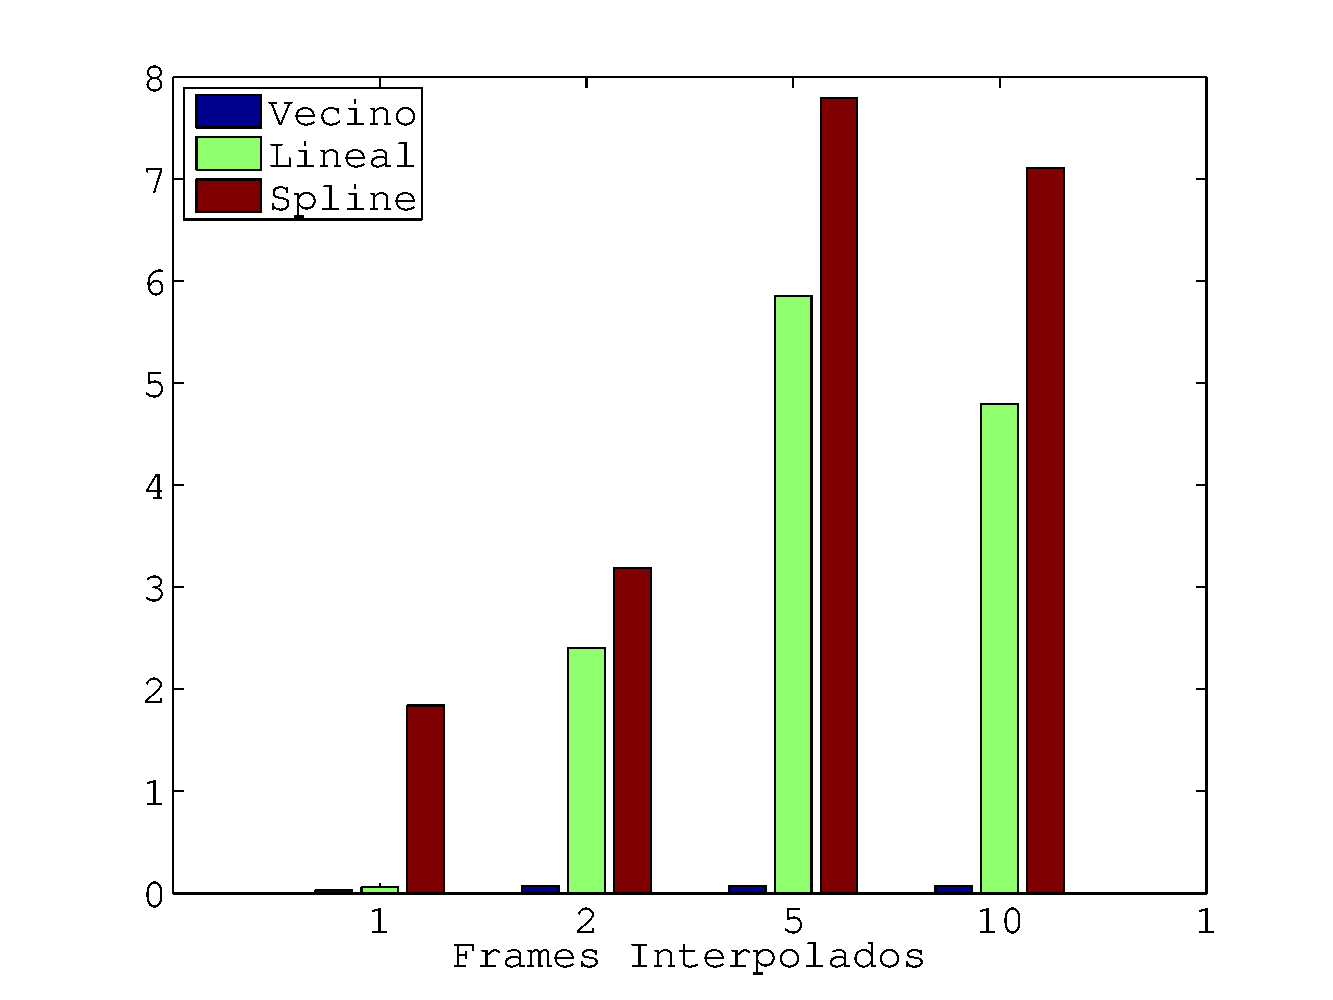
\includegraphics[width=.5\textwidth]{min_methods-camara_movil-imagen_fija.pdf}
    }
    \caption{Est\'adisticas ECM - Comparativa de M\'etodos}
    \label{fig:movil-fija_methods-mse_estadisticas}
\end{figure}

\par Del an\'alisis del valor medio del error, observamos que el comportamiento
de los 3 m\'etodos es similar a medida que se var\'ian la cantidad de frames
interpolados, aunque se observa como en la media el m\'etodo del vecino comienza
a tener una media menor que splines y lineal. De hecho, si bien splines es
casi siempre el m\'etodo con menor ECM medio (salvo para el caso de 10 frames
interpolados, donde est\'a muy cerca del vecino), pero comienza a tener cada
vez una diferencia menor al interpolarse una mayor cantidad de frames.

\par En la misma corriente de an\'alisis, se observa como el ECM medio m\'etodo
lineal tiende a crecer m\'as r\'apidamente que el m\'etodo del vecino o splines.
Estos comportamientos se ven reflejados tambi\'en en el error m\'aximo cometido
por las interpolaciones, pero no as\'i en el caso del error m\'inimo, donde
claramente el hecho de tener un frame interpolado inmediato siguiente a un frame
original como la copia de este genera un error m\'inimo m\'as peque\~no. Los
m\'etodos lineal y spline no parecieran interpolar estos frames cercanos a los
frames originales tan bien como el vecino m\'as cercano, pero parecieran ganarle
en los frames m\'as distantes. De hecho, esto explicar\'ia porque los picos
del m\'etodo del vecino (mencionados hace un par de p\'arrafos) son m\'as
intensos (mayores en casos de picos altos y menores en caso de bajos) que sus
alternativas.

\par Por \'ultimo, se presenta una comparativa de los videos comparadores para
un mismo frame en la figura \ref{fig:movil-fija_heatmap}. Si bien en el mismo
observamos que no hay diferencias muy grandes en cuanto a las diferencias entre
los cuadros originales e interpolados (salvo quiz\'as en cuanto a las sombras
de la figura), donde los 3 casos muestran como los contornos de la figura son
los que m\'as error tienen. Tambi\'en es interesante observar las diferencias
entre los cuadros interpolados de los 3 m\'etodos. Existen claras diferencias
entre el vecino m\'as cercano y sus contrapartes m\'as ''inteligentes''\footnote{Desde
el punto de vista de que tratan de realizar alg\'un proceso de los frames para
aproximar al movimiento.}.

\begin{figure}[H]
    \centering
    \subfloat[][Spline (video entero)]{
        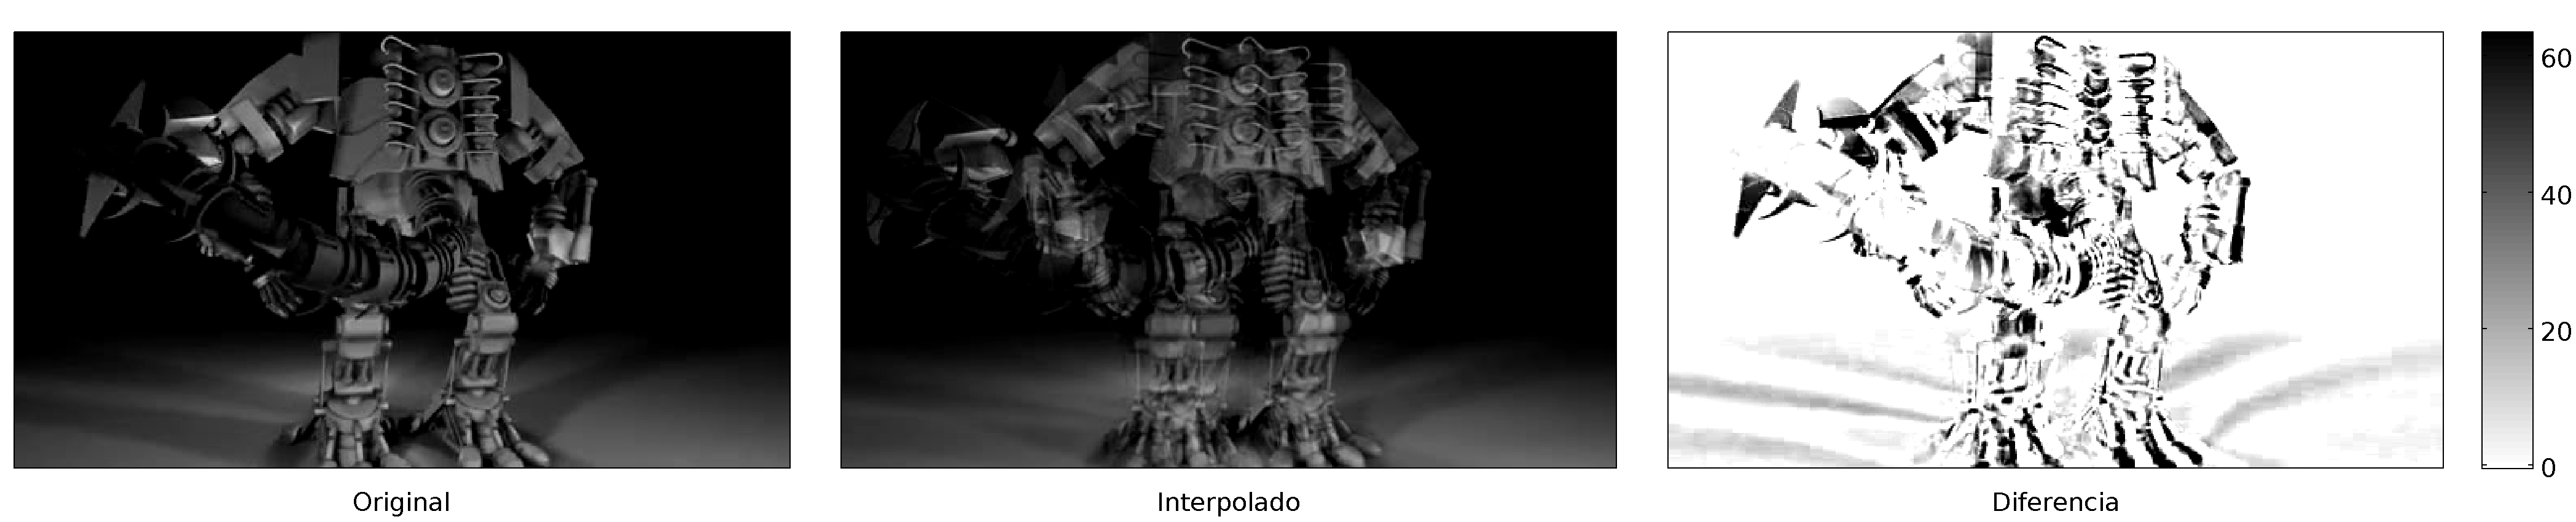
\includegraphics[width=\textwidth]{camara_movil-imagen_fija-spline-k10.png}
    }\\
    \subfloat[][Interpolaci\'on Lineal]{
        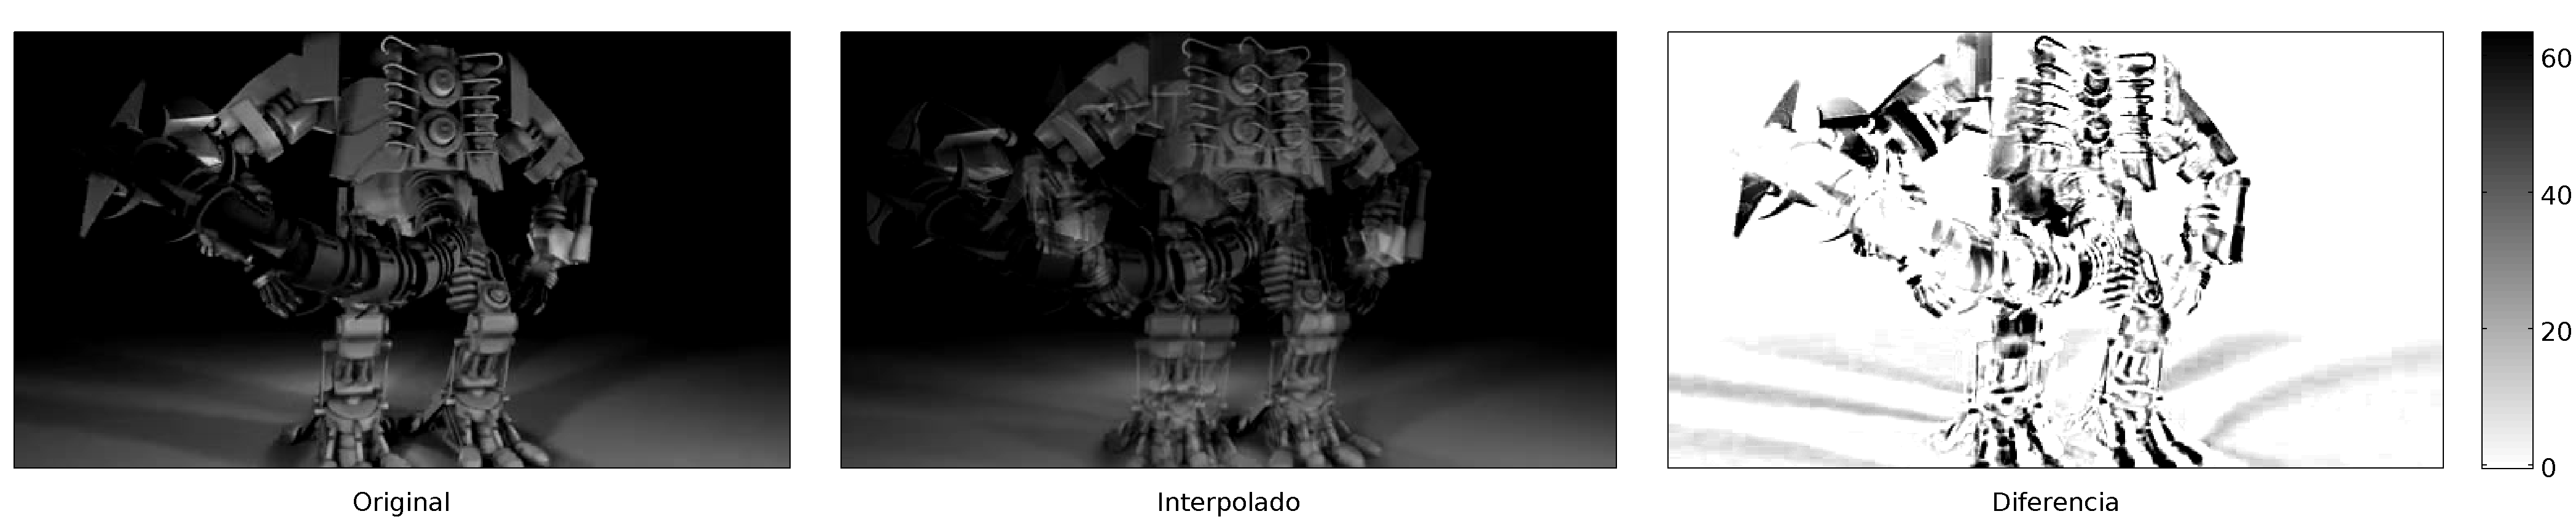
\includegraphics[width=\textwidth]{camara_movil-imagen_fija-lineal-k10.png}
    }\\
    \subfloat[][Vecino m\'as Cercano]{
        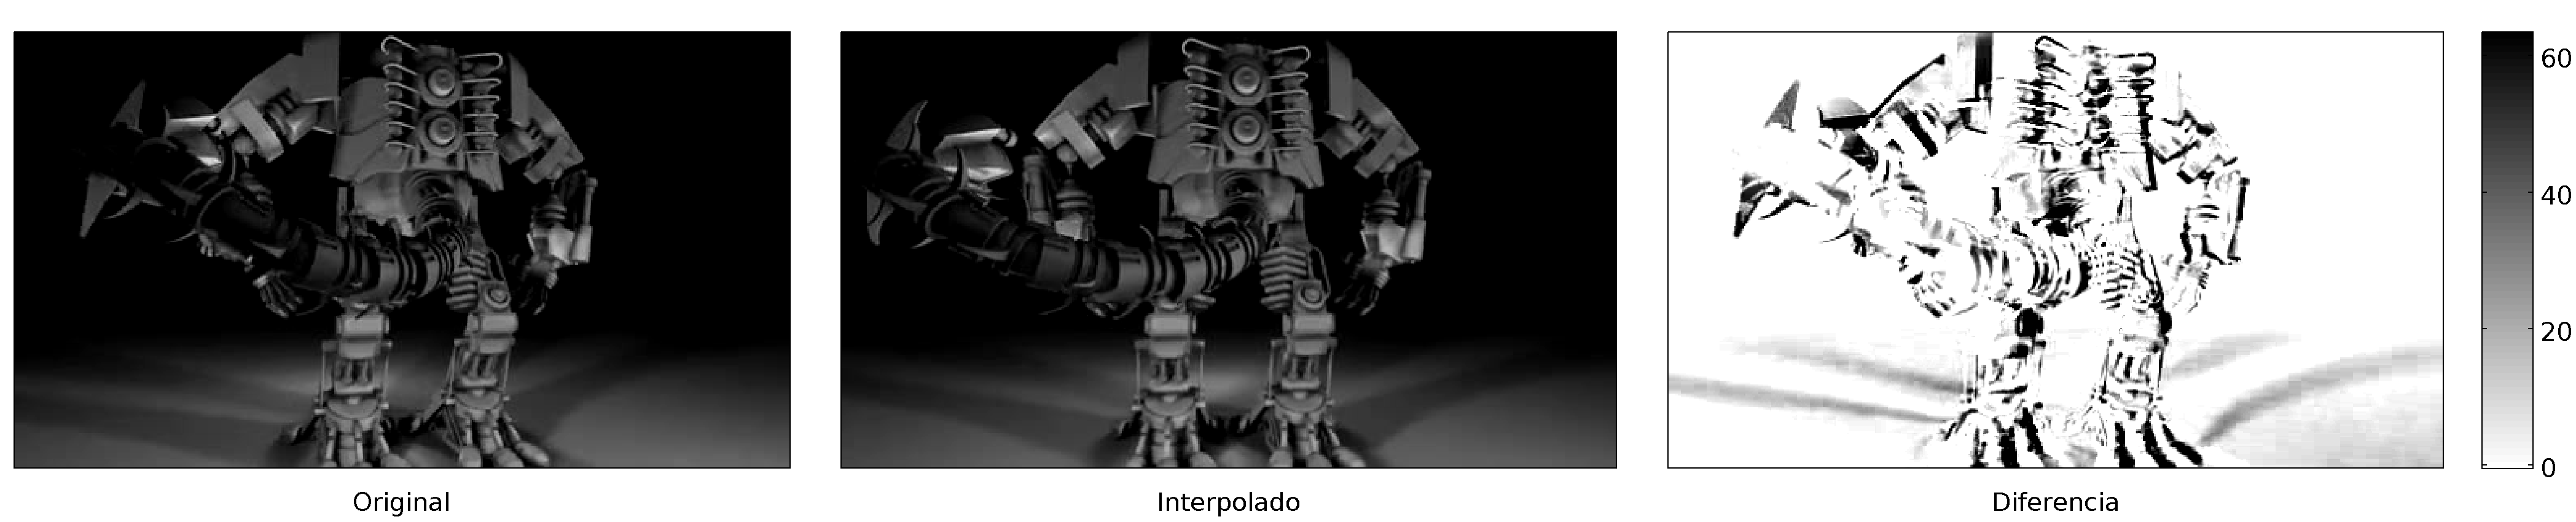
\includegraphics[width=\textwidth]{camara_movil-imagen_fija-vecino-k10.png}
    }
    \caption{Captura del mismo frame de Videos comparativos para interpolaci\'on de 10 frames}
    \label{fig:movil-fija_heatmap}
\end{figure}

%---------------------------------------------------------------
\subsubsection{Conclusiones}
\par A lo largo de este experimento volvimos a encontrarnos con algunos
resultados previamente vistos: el tama\~no de bloque en el m\'etodo de spline
no parece ser siginficativo, el m\'etodo del vecino m\'as cercano pareciera
comportarse mejor/tener menos error para pocos frames interpolados, y nuevamente
se v\'e el comportamiento oscilante de los m\'etodos entre los frames originales
sobre los que se interpola.

\par De hecho, algo nuevo que se vi\'o es la tendencia de crecimiento m\'as
alta para el ECM medio en funci\'on de los frames interpolados del m\'etodo
lineal, y significativamente m\'as baja para splines y vecino m\'as cercano; al
punto de que al transicionar desde 1 frame a 10 frames, se pasa de tener un
vecino m\'as cercano con mayor ECM a que la interpolaci\'on lineal sea la que
cometa el mayor error promedio.

\par An\'alizando un poco el dominio del video, tambi\'en conclu\'imos que son
las mismas cosas que en el experimento previo las que hacen estimar de peor
manera a los m\'etodos: el movimiento. Aunque en este caso particular, pudimos
descubrir una nueva caracter\'istica que asocia el error a los colores y
tonalidades.  Es una hip\'otesis a plantear que probablemente el error cometido
ser\'ia menor si toda la imagen tuviera menos/m\'as brillo (es decir, comenzar
a saturar la tonalidad de todos los p\'ixeles). Esto se vi\'o al analizar que
el error m\'as amplio proven\'ia de la estimaci\'on de los contornos de la
figura en cada frame, y no tanto del resto de su cuerpo.

\par Tambi\'en fue interesante encontrar un caso donde, seg\'un nuestra forma
de decidir para el caso del vecino m\'as cercano que frame utilizar en caso de
estar equidistantes de los frames originales, se afectase el error obtenido de
manera notoria (al menos para las m\'etricas, ya que para el ojo humano no lo
es\footnote{Al menos para los ojos arruinados de los autores, que est\'an hace
3 noches escribiendo frenet\'icamente delante de un monitor.}).

\par Para finalizar, quedar\'ia dar una opini\'on de los m\'etodos aplicados
desde la subjetividad de los espectadores humanos. Nuevamente, como en el
caso de \emph{c\'amara fija, im\'agen m\'ovil}, nos encontramos conque el
m\'etodo del vecino no nos resulta aceptable, o al menos no tanto como los otros
dos. De hecho, utilizar este m\'etodo simplemente da un efecto de \emph{lag} o
retraso, y no da la sensaci\'on de un movimiento sino m\'as bien una sucesi\'on
de im\'agenes. En cuanto a los m\'etodos restantes, no se han distinguido cambios
en cuanto al resultado de uno y el otro, con lo cual en caso de tener que elegir
uno se tomar\'ia la interpolaci\'on lineal, por ser esta menos costosa
computacionalmente hablando.
%---------------------------------------------------------------
